
\subsection{Punto 1}

\textbf{Enunciado}: \textsl{Analizar que función cumple y como opera el subcircuito compuesto por $R_{12}$ a $R_{17}$, $C_{16}$ y $U_{3}A$. Luego incluir $R_{S}$. ¿Qué características tiene éste subcircuito, por ejemplo, su transferencia, su ancho de banda, su dependencia de las especificaciones del amplificador operacional $TL082$, de sus fuentes de alimentación, de la temperatura, de la tolerancia y tecnología de los resistores con los que se lo implemente, etc.}


\vspace{1.5cm}


Se explica en detalle en \sectref{section:modelo_operacional}.



\subsection{Punto 2}

\textbf{Enunciado}: \textsl{Analizar qué función cumple y como opera el subcircuito compuesto por $R_{18}$ a $R_{19}$, $C_{15}$ y $U_{3}B$. ¿Qué características tiene éste subcircuito, por ejemplo, su transferencia, su ancho de banda, su dependencia de las especificaciones del amplificador operacional $TL082$, de sus fuentes de alimentación, de la temperatura, de la tolerancia y tecnología de los resistores con lo que se lo implemente, etc. ($R_{18}$ puede variarse desde $0 \si[per-mode=symbol]{\ohm}$ a $18 \si[per-mode=symbol]{\kilo\ohm}$).}


\vspace{1.5cm}


\textcolor{red}{\textbf{COMPLETAR!!}}



\clearpage


\subsection{Punto 3}

\textbf{Enunciado}: \textsl{Analizar qué función cumple y cómo opera el subcircuito compuesto por $R_{20}$ a $R_{23}$ y $Q_{7}$-$Q_{9}$-$Q_{10}$-$Q_{11}$. ¿Qué características tiene éste subcircuito?.}

\vspace{1.5cm}

La ganancia global del amplificador, por tratarse de un circuito realimentado, tomando los valores calculados anteriormente para $a$ y $f$ en la sección~\sectref{calculation_of_f}, será:

\begin{equation}
\boxed{ A = \frac{a}{1 + a \cdot f} = \frac{6718}{1 + 6718 \cdot 0.035} \approx 28.5 }
\end{equation}

El valor es prácticamente igual a $\frac{1}{f} \approx 28.6$, dado que se verifica muy bien la condición $a \gg 1$.


\vfill

\clearpage


\subsection{Punto 4}

\textbf{Enunciado}: \textsl{Analizar el subcircuito que proporciona la tensión de referencia. ¿Cómo funciona y qué características tiene? Por ejemplo: hallar por cálculo y por simulación el valor de la tensión de referencia y su dependencia de la variación de la tensión de entrada $V_{1}$, de la temperatura ambiente y de la corriente que pueda entregar éste subcircuito a otros subcircuitos que alimente. Consultar las hojas de datos de todos sus componentes, en especial el $TL431$.}


\vspace{1.5cm}



El circuito de la referencia de tensión se analiza cualitativamente y con algunos resultados por simulación en la sección~\sectref{section:voltage_reference}.\\


\subsection{Punto 5}

\textbf{Enunciado}: \textsl{Analizar el subcircuito compuesto por $Q_{4}$ y $Q_{5}$. Por ejemplo: con que nombre es conocida su topología, comprobar si es una topología que emplea realimentación, qué características funcionales tiene este subcircuito, que valores de impedancia presente a los otros circuitos que alimente, cual es la transferencia de este subcircuito (variable de salida / variable de entrada), cuál es su ancho de banda, etc.}


\vspace{1.5cm}



El circuito formado por los dos transistores, $Q_{4}$ y $Q_{5}$, se trata de un par compuesto Sziklai. En la sección~\sectref{section:sziklai} hacemos un análisis del mismo.\\


\clearpage




\subsection{Punto 6}

\textbf{Enunciado}: \textsl{¿Cuál es el rango de la tensión de salida de la fuente considerando que $R_{9}$ puede variar desde $0 \si[per-mode=symbol]{\ohm}$ a $90 \si[per-mode=symbol]{\kilo\ohm}$? (Tomar $R_{L} = 1 \si[per-mode=symbol]{\mega\ohm}$).}

\vspace{1.5cm}


En la figura~\figref{fig:fig_p6_output_voltage} se muestra el gráfico de la tensión de salida en modo de regulación de tensión en función de la resistencia del resistor $R_{9}$, el gráfico se obtuvo realizando una simulación paramétrica con $R_{L} = 1 \si[per-mode=symbol]{\mega\ohm}$, con el comando \textbf{SPICE} \textit{.step}, y luego se exportó el resultado y se graficó en \textbf{MATLAB}. En el gráfico se puede apreciar que, como se espera según lo calculado, el crecimiento es lineal con $R_{9}$, entre valores muy cercanos a los nominales de $1 \si[per-mode=symbol]{\volt}$ y $10 \si[per-mode=symbol]{\volt}$.




\vfill

\clearpage

\begin{figure}[H] %htb
\begin{center}
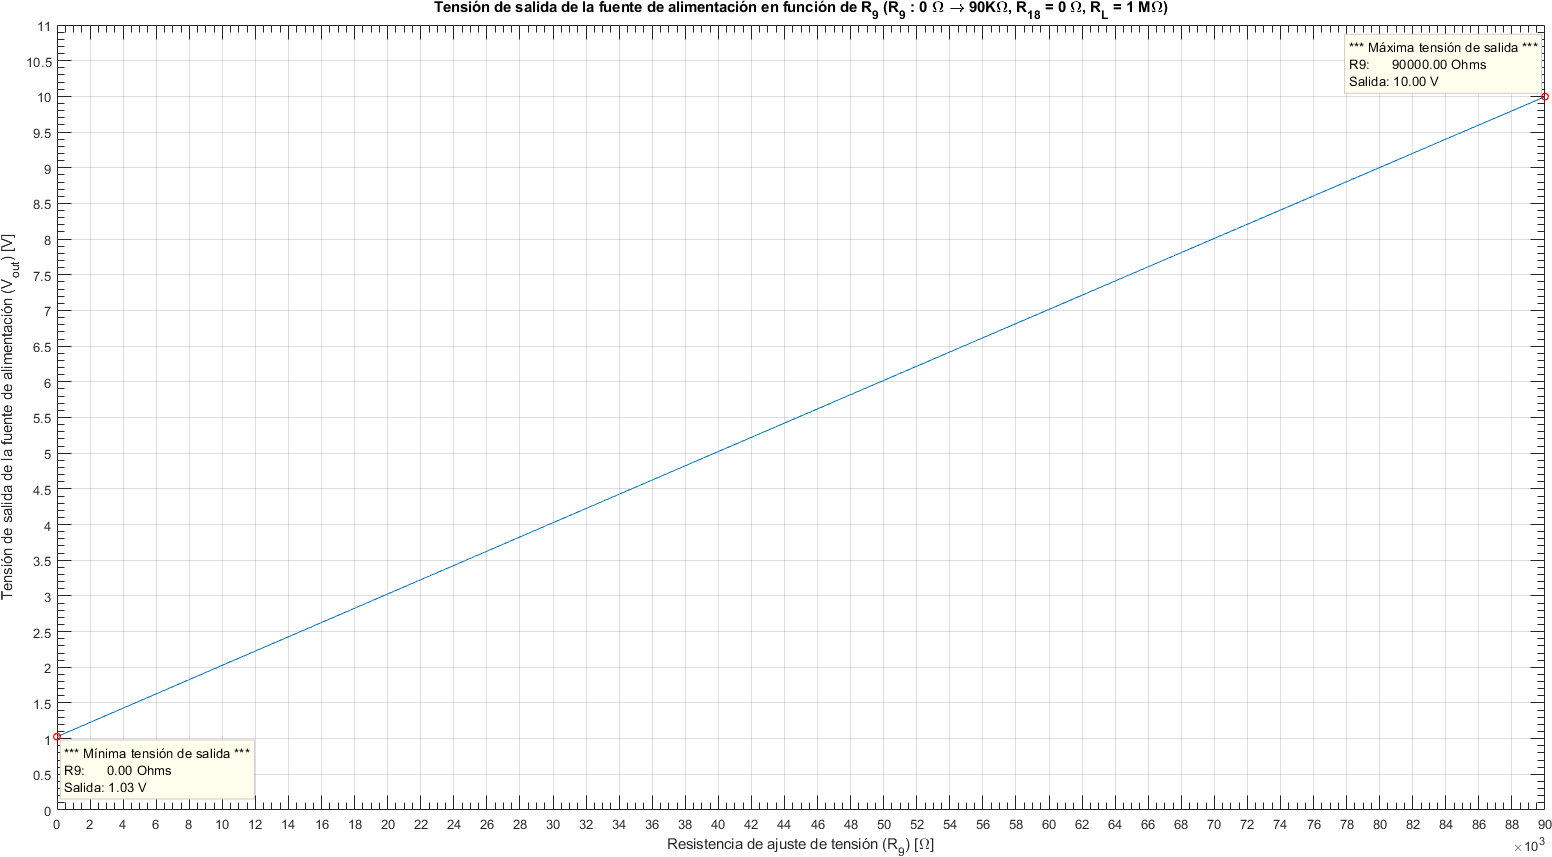
\includegraphics[width=1.2 \textwidth, angle=90]{./img/preguntas/p6.png}
\caption{\label{fig:fig_p6_output_voltage}\footnotesize{Tensión de salida, $V_{o}$, en función de $R_{9}$, con esta variando entre $0 \si[per-mode=symbol]{\ohm}$ y $90 \si[per-mode=symbol]{\kilo\ohm}$.}}
\end{center}
\end{figure}



\clearpage

\subsection{Punto 7}

\textbf{Enunciado}: \textsl{¿Cuál es el rango la corriente de salida de la fuente considerando que $R_{18}$ puede variar desde $0 \si[per-mode=symbol]{\ohm}$ a $18 \si[per-mode=symbol]{\kilo\ohm}$? (Tomar $R_{L} = 0 \si[per-mode=symbol]{\ohm}$).}

\vspace{1.5cm}

El factor de amortiguamiento, $DF$ (damping factor), es la relación entre la impedancia especificada de la carga, $8 \si[per-mode=symbol]{\ohm}$ en este caso, y la impedancia de salida del amplificador, ambas consideradas como resistivas puras, a frecuencias medias, se tiene entonces:


\begin{equation}
\boxed{ DF = \frac{R_{L}}{R_{o}} = \frac{8 \si[per-mode=symbol]{\ohm}}{29.6 \si[per-mode=symbol]{\milli\ohm}} \approx 270.3 }
\end{equation}


\vfill

\clearpage



\subsection{Punto 8}

\textbf{Enunciado}: \textsl{¿Cuál es el valor de la resistencia de carga $R_{L}$ que impone el límite entre el modo fuente de tensión y fuente de corriente para $R_{9} = 90 \si[per-mode=symbol]{\kilo\ohm}$ y $R_{18} = 0 \si[per-mode=symbol]{\ohm}$?.}

\vspace{1.5cm}

\label{punto8}

Para obtener la máxima tensión pico sobre la carga, debemos hacer la suposición que la misma se obtiene al límite donde los transistores del amplificador están al borde salir de modo activo directo, en general no son solo los transistores de la etapa de salida, sino que dependiendo la configuración el límite será impuesto por los transistores de mas de una etapa.\\

En particular para este amplificador podemos ver que para los ciclos positivo de la señal, lo siguiente:

\begin{equation} \label{eq:1}
\hat{V}_{L{max}} + V_{BE_{407}} + V_{BE_{405}} + \hat{V}_{R_{421_{max}}} = V_{CC}
\end{equation}

Condición que lleva a $Q_{407}$ y $Q_{405}$ al límite de la saturación, por supuesto en esta condición la distorsión por alinealidad será  máxima, pero mas allá el amplificador comenzará a recortar.

además tenemos que:

\begin{equation} \label{eq:2}
\hat{V}_{R_{421_{max}}} = \hat{I}_{L_{max}} \cdot R_{421} = \frac{\hat{V}_{L{max}}}{R_{L}}
\end{equation}

Combinando \ref{eq:1} y \ref{eq:2} tenemos:

\begin{equation} \label{eq:3}
\hat{V}_{L{max}} = \frac{V_{CC} - V_{BE_{407}} - V_{BE_{405}} }{1 + \frac{R_{421}}{R_{L}} }
\end{equation}


Pero \ref{eq:3} es una expresión trascendente , ya que $V_{BE_{405}}$ y $V_{BE_{407}}$ dependen de la corriente de colector de cada transistor. Asumiendo para el par una relación de $\beta$ veces en las corrientes, se tiene:


\begin{equation} \label{eq:3}
 \hat{I}_{C_{407_{max}}} = \frac{\hat{I}_{L_{max}}}{1 + \frac{1}{\beta_{407}} } = \frac{\hat{V}_{L_{max}}}{ R_{L} \cdot \left( 1 + \frac{1}{\beta_{407}} \right) }
\end{equation}

Podemos operar iterativamente usando las curvas de $I_{C} = f_{\left( V_{BE} \right)}$ de cada transistor, \textbf{Figura~10},\, \quotemarks{On~Voltages}, de la hoja de datos del transistor \textbf{TIP41}, apéndice~\sectref{datasheet_TIP41}, y \textbf{Figura~4}, \quotemarks{\mbox{Base-Emitter~On~Voltage}}, de la hoja de datos del transistor \textbf{BD135}, apéndice~\sectref{datasheet_BD135}, empezamos asumiendo que $V_{BE} = 0.7$ para ambos transistores, calculamos una tensión de pico máxima y con esta una corriente de colector máxima para el transistor $Q_{407}$ y de esta un nuevo valor para el $V_{BE}$, que nos permite calcular un nuevo valor para la tensión pico máxima, en este caso con una iteración es suficiente, se obtiene:

\begin{equation} \label{eq:3}
\boxed{\hat{V}_{L{max}} = 26.6 \si[per-mode=symbol]{\volt}}
\end{equation}

Para el ciclo negativo se obtiene un valor cercano, haciendo un análisis similar, pero que involucra a los transistores $Q_{406}$ y $Q_{404}$, tomamos este valor para el ciclo positivo, de todos modos es solo una aproximación. 



\vfill

\clearpage


\subsection{Punto 9}

\textbf{Enunciado}: \textsl{¿Qué hace (o para que está) cada componente, o sea, que función cumple en el circuito y justificar el valor de cada resistencia, diodo, transistor, etc?\\
En particular, respecto de la pregunta anterior, explicar que función realiza $D_{1}$ y justificar la elección de su designación como $1N4148$.}

\vspace{1.5cm}

Para calcular la máxima eficiencia del amplificador, utilizamos la definición de eficiencia:

\begin{equation}
\eta_{max} = max\left\{ \frac{P_{L}}{P_{sources}} \right\} \cdot 100\%
\end{equation}

Donde $P_{L}$ es la potencia entregada a la carga y $P_{sources}$ es la potencia entregada por las fuentes de alimentación. Se puede observar fácilmente que la potencia consumida por todos los transistores que trabajan en \textbf{clase A}, no varía, salvo al tener señal aplicada, parte de esa potencia es entregada a la siguiente etapa, pero todos los transistores, excepto los de la etapa de salida, no entregan potencia a la carga, por lo que no contribuyen a la potencia útil, solo a la consumida, con esto en mente, basta ver las corrientes de reposo de todas las ramas, excepto la de los transistores de potencia, para obtener la parte fija del consumo en la fuente. Luego para ver el cuando se da el caso de mayor eficiencia, se ve fácilmente que será cuando se entregue la máxima potencia a la carga.\\


Usando la expresión general de la potencia máxima en un \textbf{clase AB}, pero con correcciones para tener en cuenta el consumo de potencia en las primeras etapas en \textbf{clase A} y la potencia disipada en las resistencias de emisor de la etapa de salida, llamando $I_{cA}$ a la corriente que circula por las ramas de las primeras etapas, y usando los valores máximos obtenidos en la sección~\sectref{max_pot}, tenemos:


\begin{equation*}
\eta_{max} = \frac{ \frac{ \hat{I}_{L{max}} \cdot \hat{V}_{L{max}} }{2}   }{  \frac{ 2 \cdot \hat{I}_{L{max}} \cdot V_{CC}  }{ \pi } + \left( V_{CC} + V_{SS} \right) \cdot I_{cA} + \hat{I}_{L{max}} \cdot R_{421}  } \cdot 100\%
\end{equation*}\\


\begin{equation}
\boxed{ \eta_{max} = \frac{ \frac{ 3.33 \si[per-mode=symbol]{\ampere}  \cdot 26.6 \si[per-mode=symbol]{\volt} }{2}   }{  \frac{ 2 \cdot  3.33 \si[per-mode=symbol]{\ampere} \cdot 30 \si[per-mode=symbol]{\volt}  }{ \pi } + 60 \si[per-mode=symbol]{\volt} \cdot 9.25 \si[per-mode=symbol]{\milli\ampere} + 3.33 \si[per-mode=symbol]{\ampere} \cdot 0.47 \si[per-mode=symbol]{\ohm}  } \cdot 100\% \approx 67.4 \% }
\end{equation}




\vfill

\clearpage


\subsection{Punto 10}

\textbf{Enunciado}: \textsl{¿Qué tecnología, tolerancia, capacidad de disipación de potencia, estabilidad con la temperatura, tensión y corriente de operación máxima y pulsante, características mecánicas, apartamiento de su valor nominal por envejecimiento, etc, debe tener cada componente considerando una implementación física de éste circuito?.}

\vspace{1.5cm}

\subsubsection{Tamaño de los disipadores para cada transistor (resistencia térmica disipador-ambiente)}
\label{thermal_calculation}

Primero determinamos de los puntos de trabajo calculados en la sección~\sectref{qpoint}, las potencias disipadas en cada uno de los transistores de señal y potencia media, los resultados se resumen en el cuadro~\tableref{table:table_powers}


%% \noindent
%% \begin{center}
 
%%\begin{spacing}{1}  
\begin{table}[H]  %%\centering
    
    \setlength\arrayrulewidth{1.5pt}
    \arrayrulecolor{white}
    \def\clinecolor{\hhline{|>{\arrayrulecolor{white}}-%
    >{\arrayrulecolor{white}}|-|-|-|-|-|}}
\resizebox{0.8 \textwidth}{!}{% 
       
\begin{tabularx}{1 \textwidth}%
    {|
    >{\columncolor{white} \centering\arraybackslash}m{0.29\linewidth}
     |
    >{\columncolor{white} \centering\arraybackslash}m{0.14\linewidth}
     |
    >{\columncolor{white} \centering\arraybackslash}m{0.14\linewidth}
     |
    >{\columncolor{white} \centering\arraybackslash}m{0.14\linewidth}
     |
    >{\columncolor{white} \centering\arraybackslash}m{0.14\linewidth}
     |
    >{\columncolor{white} \centering\arraybackslash}m{0.14\linewidth}
     |
    }
    \rowcolor{HeadersColor} \cellcolor{white} \thead{}  & \thead{$Q_{402}$} & \thead{$Q_{403}$} & \thead{$Q_{404}$} & \thead{$Q_{405}$} & \thead{$Q_{406}$} \\
    
    \hhline{|-|-|-|-|-|}
    \rowcolor{gray!20} \cellcolor{gray!40} $I_{C}$ [$\si[per-mode=symbol]{\milli\ampere}$] & $0.54$ & $8.66$ & $9$ & $6$ & $5.5$  \\
    \hhline{|-|-|-|-|-|}
    \rowcolor{gray!20} \cellcolor{gray!40} $V_{CE}$ [$\si[per-mode=symbol]{\volt}$] & $26.1$ & $1.8$ & $27.95$ & $29.4$ & $29.4$  \\
    \hhline{|-|-|-|-|-|}
    \rowcolor{Butter!20} \cellcolor{gray!40}  $P_{D}$ [$\si[per-mode=symbol]{\watt}$] & $14.1 \si[per-mode=symbol]{\milli}$ & $15.6 \si[per-mode=symbol]{\milli}$ & $251 \si[per-mode=symbol]{\milli}$ & $228 \si[per-mode=symbol]{\milli}$ & $228 \si[per-mode=symbol]{\milli}$ \\
    \hhline{|-|-|-|-|-|}
    \rowcolor{gray!20} \cellcolor{gray!40} \thead{\cellcolor{gray!40} \color{black} $P_{D_{max}}^{*}$ [$\si[per-mode=symbol]{\watt}$] } & $625 \si[per-mode=symbol]{\milli}$ & $625 \si[per-mode=symbol]{\milli}$ & $1.25$ & $1.25$ & $1.25$  \\
    \hhline{|-|-|-|-|-|}  
    \rowcolor{gray!20} \cellcolor{gray!40} \thead{\cellcolor{gray!40} \color{black} $\theta_{ja}^{*}$ [$\si[per-mode=symbol]{\celsius\per\watt}$] } & $200$ & $200$ & $100$ & $100$ & $100$  \\
    \hhline{|-|-|-|-|-|}  
    \rowcolor{gray!20} \cellcolor{gray!40} \thead{\cellcolor{gray!40} \color{black} $\theta_{jc}^{*}$ [$\si[per-mode=symbol]{\celsius\per\watt}$] } & $83.3$ & $83.3$ & $10$ & $10$ & $10$  \\
    \hhline{|-|-|-|-|-|}     
       
    \end{tabularx}}
	\caption{\footnotesize{Potencia disipada en los transistores de señal y media potencia.}}
	\label{table:table_powers}
\end{table}
%%\end{spacing}

%% \end{center}

\footnotesize{
$\left(*\right)$ Los datos se tomaron de las correspondientes hojas de datos.
}\\\\


Para todos los transistores que trabajan en \textbf{clase A}, $Q_{402}$, $Q_{403}$ y $Q_{404}$, las potencias disipadas se calcularon simplemente como $V_{CE} \cdot I_{C}$, ya que esto corresponde a la máxima potencia disipada en el transistor, que se da cuando no hay señal en el mismo.\\

Para los transistores $Q_{405}$ y $Q_{406}$, los drivers de los pares compuestos que integran la etapa de salida en \textbf{clase AB}, se hizo las siguientes  suposiciones simplificadoras, que la tensión \mbox{colector-emisor} en los mismos coincide con la de los transistores de salida y que por los mismos circula una corriente que es $\beta$ veces menor que en los transistores de salida, de esta forma la potencia termina siendo $\beta$ veces menor que en estos. De todas formas se trata de unas suposiciones conservadoras.\\

Para los dos transistores de salida, la potencia máxima disipada se calcula como:

\begin{equation}
      P_{C_{max_{Q_{407}}}} = P_{C_{max_{Q_{4088}}}} = \frac{{V_{CC}}^2}{{\pi}^2 \cdot R_{L}} = 11.4 \si[per-mode=symbol]{\watt}
\end{equation}\\

Y se obtiene entonces para los transistores drivers de los pares:

\begin{equation}
P_{C_{max_{Q_{405}}}} = P_{C_{max_{Q_{406}}}} = \frac{P_{C_{max_{Q_{7}}}}}{\beta_{407}} = \frac{11.4 \si[per-mode=symbol]{\watt}}{50} = 228 \si[per-mode=symbol]{\milli\watt}
\end{equation}\\

Para determinar la necesidad de un disipador térmico en cada uno de los transistores, suponemos su operación sin el mismo y planteamos el circuito térmico correspondiente. Para este planteo se necesitan también los siguientes parámetros:

\begin{enumerate}
\item[$\bm{T_{j_{max}}}$] Temperatura máxima de operación de la juntura del transistor ($150 \si[per-mode=symbol]{\celsius}$ para todos los transistores analizados).
\item[$\bm{T_{j_{e}}}$] Temperatura de operación estimada de la juntura del transistor.
\item[$\bm{T_{a}}$] Temperatura ambiente (tomamos $40 \si[per-mode=symbol]{\celsius}$ como un caso de un circuito encerrado en un gabinete).
\item[$\bm{\theta_{ja}}$] Resistencia térmica de la juntura del transistor al ambiente.\\
\end{enumerate}


Entonces solo tenemos una fuente de potencia, $P_{D}$ (modelada por una fuente de corriente) circulando por la resistencia térmica $\theta_{ja}$ (modelada como una resistencia eléctrica), con lo que la temperatura (modelada por tensión) que se desarrolla sobre la juntura se suma a la temperatura ambiente (modelada por una fuente de tensión), con lo que nos queda:


\begin{equation} \label{eq:thermal_ambient}
T_{j_{e}} = P_{D} \cdot \theta_{ja} + T_{a}
\end{equation}\\

Nos queda para cada uno de los transistores de señal y para los drivers de los pares:

\begin{enumerate}
\item[$\bm{Q_{402}}$] $T_{j_{e_{402}}} = 41.2 \si[per-mode=symbol]{\celsius} $ 
\item[$\bm{Q_{403}}$] $T_{j_{e_{403}}} = 41.3 \si[per-mode=symbol]{\celsius} $ 
\item[$\bm{Q_{404}}$] $T_{j_{e_{404}}} = 65.1 \si[per-mode=symbol]{\celsius} $
\item[$\bm{Q_{405}}$] $T_{j_{e_{405}}} = 62.8 \si[per-mode=symbol]{\celsius} $
\item[$\bm{Q_{406}}$] $T_{j_{e_{406}}} = 62.8 \si[per-mode=symbol]{\celsius} $
\item[$\bm{Q_{407}}$] $T_{j_{e_{407}}} = 62.8 \si[per-mode=symbol]{\celsius} $
\item[$\bm{Q_{408}}$] $T_{j_{e_{408}}} = 62.8 \si[per-mode=symbol]{\celsius} $
\end{enumerate}

Podemos ver que ninguno de los transistores supera la máxima temperatura de trabajo, con lo que concluimos que no necesitan disipador térmico.\\

Para los transistores de salida, ambos son el mismo tipo de transistor, obtenemos las resistencias térmicas de la \textbf{figura 7}, \quotemarks{Power Derating} de la hoja de datos del transistor \textbf{TIP41}, apéndice~\sectref{datasheet_TIP41}. Obtenemos:\\

$\theta_{ja_{Q_{407}}} = \theta_{ja_{Q_{408}}} = 60 \si[per-mode=symbol]{\celsius\per\watt}$ y $\bm{\theta_{jc_{Q_{407}}}} = \bm{\theta_{jc_{Q_{408}}}} = 1.9 \si[per-mode=symbol]{\celsius\per\watt} $.\\

Si aplicamos la expresión~\ref{eq:thermal_ambient} nuevamente, obtenemos para ambos transistores de salida:\\

$T_{j_{e_{407}}} = T_{j_{e_{408}}} =  724 \si[per-mode=symbol]{\celsius} $\\

Muy por encima de la temperatura máxima de trabajo para la juntura, con lo que es necesario un disipador térmico. Para calcular la resistencia térmica máxima del disipador que se necesita, se plantea un circuito térmico, pero ahora conteniendo las resistencias térmicas de la juntura al encapsulado, del encapsulado al disipador y del disipador al ambiente, esta última es la que se necesita determinar, en la figura~\figref{fig:fig_thermal_circuit} se muestra el circuito térmico completo.


\begin{figure}[H] %htb
\begin{center}
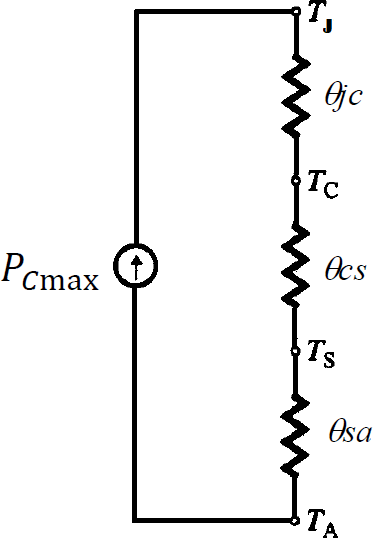
\includegraphics[width=0.35 \textwidth, angle=0]{./img/desarrollo/thermal_circuit.png}
\caption{\label{fig:fig_thermal_circuit}\footnotesize{Circuito térmico para los transistores de salida.}}
\end{center}
\end{figure}

Del planteo de este circuito se despeja la expresión para la resistencia térmica del disipador, $\theta_{sa}$, se obtiene:

\begin{equation}
\theta_{sa} = \frac{T_{J} - T_{a}}{P_{C_{max}}} - \theta_{jc} - \theta_{cs}
\end{equation}


Donde $\theta_{jc}$ ya se obtuvo de las hojas de datos y $\theta_{cs}$, la resistencia térmica del encapsulado al disipador, depende del montaje mecánico que se realiza del transistor sobre el disipador, el mismo puede ser con mica, grasa siliconada, o ambas, el transistor se puede justar mas o menos sobre la superficie del disipador, etc. Teniendo en cuenta estas variantes se estima que $1 \si[per-mode=symbol]{\celsius\per\watt} \leq \theta_{cs} \geq 0.5 \si[per-mode=symbol]{\celsius\per\watt} $, tomamos $1 \si[per-mode=symbol]{\celsius\per\watt}$, el peor caso. Obtenemos entonces para los transistores de salida:

\begin{equation}
\theta_{sa_{max}} = \frac{T_{J} - T_{a}}{P_{C_{max}}} - \theta_{jc} - \theta_{cs} = \frac{150 \si[per-mode=symbol]{\celsius} - 40 \si[per-mode=symbol]{\celsius}   }{11.4  \si[per-mode=symbol]{\watt} } - 1.9 \si[per-mode=symbol]{\celsius\per\watt} - 1 \si[per-mode=symbol]{\celsius\per\watt} \approx 6.8 \si[per-mode=symbol]{\celsius\per\watt}\\ \\
\end{equation}

Con lo que solo necesitamos disipadores para los transistores de salida que cumplan:

\begin{center}
\begin{equation}
\boxed{ \theta_{sa} \leq 6.8 \si[per-mode=symbol]{\celsius\per\watt} }
\end{equation}
\end{center}

\clearpage

\subsubsection{Disipador comercial que podría utilizarse para construir un prototipo funcional}

En la sección anterior calculamos la resistencia térmica que debe tener el disipador térmico de los transistores de salida, se encontró que, $\theta_{sa} \leq 6.8 \si[per-mode=symbol]{\celsius\per\watt}$, usando este valor como referencia se seleccionó un disipador que sería adecuado, el mismo se muestra en la figura~\figref{fig:fig_thermal_dissipator}, tiene $\theta_{sa} = 5.1 \si[per-mode=symbol]{\celsius\per\watt}$, es el modelo \textbf{6225M ZD-5}.

\begin{figure}[H] %htb
\begin{center}
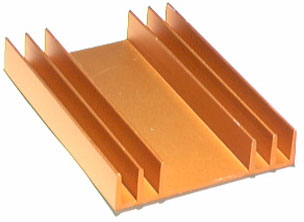
\includegraphics[width=0.6 \textwidth, angle=0]{./img/desarrollo/10b_6225M_ZD_5.png}
\caption{\label{fig:fig_thermal_dissipator}\footnotesize{Disipador térmico seleccionado (\textbf{6225M ZD-5}).}}
\end{center}
\end{figure}


\subsubsection{Comparación con los disipadores utilizados originalmente por Turner}

No pudimos encontrar información acerca del valor de la resistencia térmica de los disipadores usados originalmente, pero de las fotos que hay disponibles, los disipadores eran tipo \textbf{U}, el tamaño y el largo aparente de las aletas hacen parecer que tiene una masa metálica aproximadamente del mismo tamaño, pero no hay mucho mas que podamos decir, salvo que es probable que los disipadores hayan sido sobre-dimensionados al tratarse de un producto comercial, y que probablemente la temperatura interna del gabinete sea superior a la que nosotros consideramos.




\clearpage


\subsection{Punto 11}

\textbf{Enunciado}: \textsl{Calcular la ganancia de lazo \quotemarks{af} para el lazo de tensión y para el lazo de corriente, comparando en ambos casos con respecto a 1, o sea, ¿Resulta \quotemarks{af} mucho mayor que $1$? Considerar esto para frecuencias del orden de entre $0 \si[per-mode=symbol]{\hertz}$ y $100 \si[per-mode=symbol]{\hertz}$.}

\vspace{1.5cm}

\clearpage

\subsubsection{Punto de reposo hallado por simulación}

En la figura~\figref{fig:fig_simulated_qpoint} se muestra lo hallado por simulación para el circuito. Vemos una gran similitud con los valores calculados anteriormente, figura~\figref{fig:fig_calculated_qpoint}, aunque hubo que cambiar el valor de $PS_{401}$ con respecto al calculado para acercarnos lo más posible a $0 \si[per-mode=symbol]{\volt}$ en la salida, y también se tuvo que cambiar el valor de $PS_{402_{A}}$ y $PS_{402_{B}}$ para asegurar $10 \si[per-mode=symbol]{\milli\ampere}$ en los colectores de $Q_{407}$ y $Q_{408}$.


\begin{figure}[H] %htb
\begin{center}
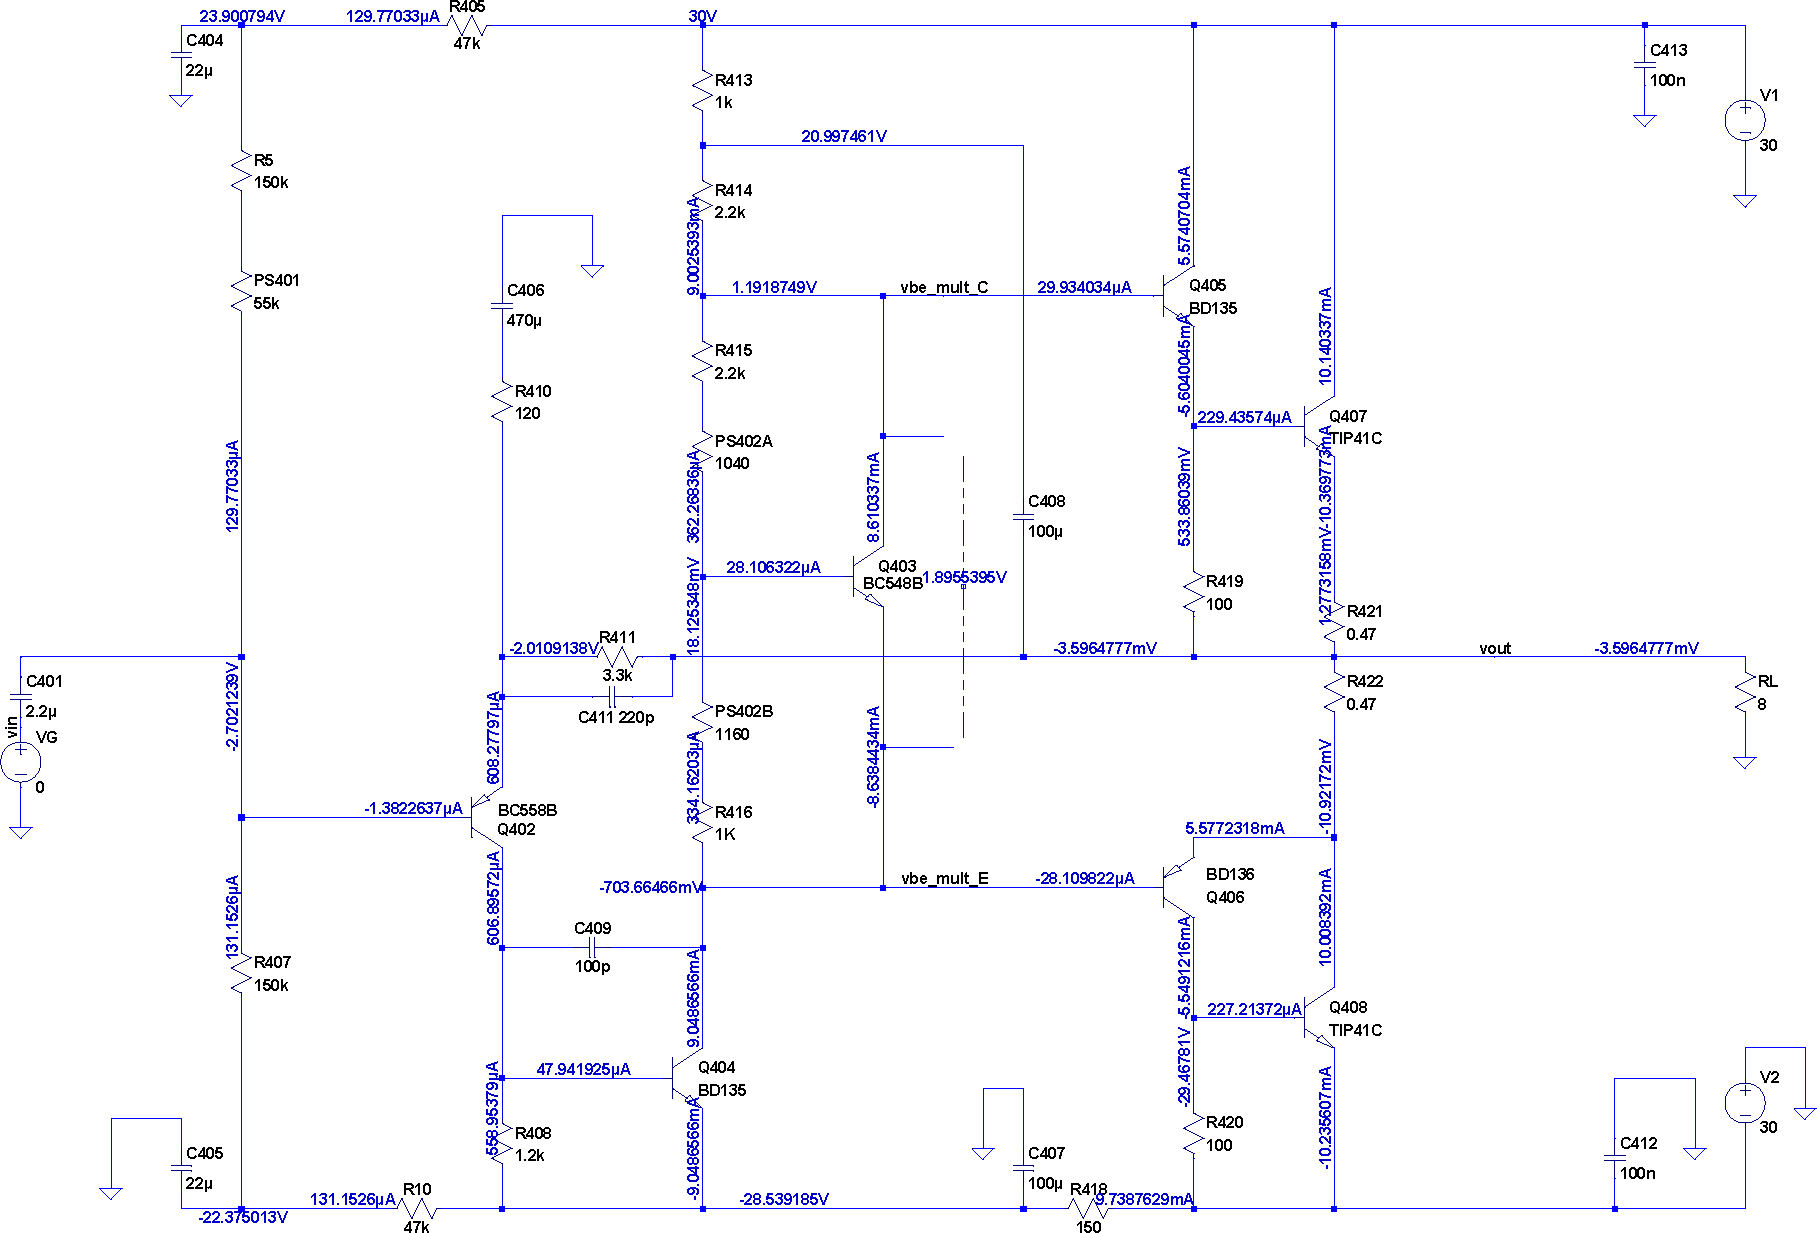
\includegraphics[width=0.9 \textwidth, angle=90]{./img/circuitos_usados/P1_P11a_qpoint.png}
\caption{\label{fig:fig_simulated_qpoint}\footnotesize{Punto de reposo del circuito hallado por simulación.}}
\end{center}
\end{figure}


\clearpage

\subsubsection{Impedancia de entrada hallada por simulación}

En la figura~\figref{fig:fig_simulated_zi} se muestra lo obtenido al simular para obtener la impedancia de entrada, el valor a frecuencias medias $86.02 \si[per-mode=symbol]{\kilo\ohm}$ se acerca bastante al valor calculado en la sección~\sectref{calculated_zi}, se había calculado $85.3 \si[per-mode=symbol]{\kilo\ohm}$.


\begin{figure}[H] %htb
\begin{center}
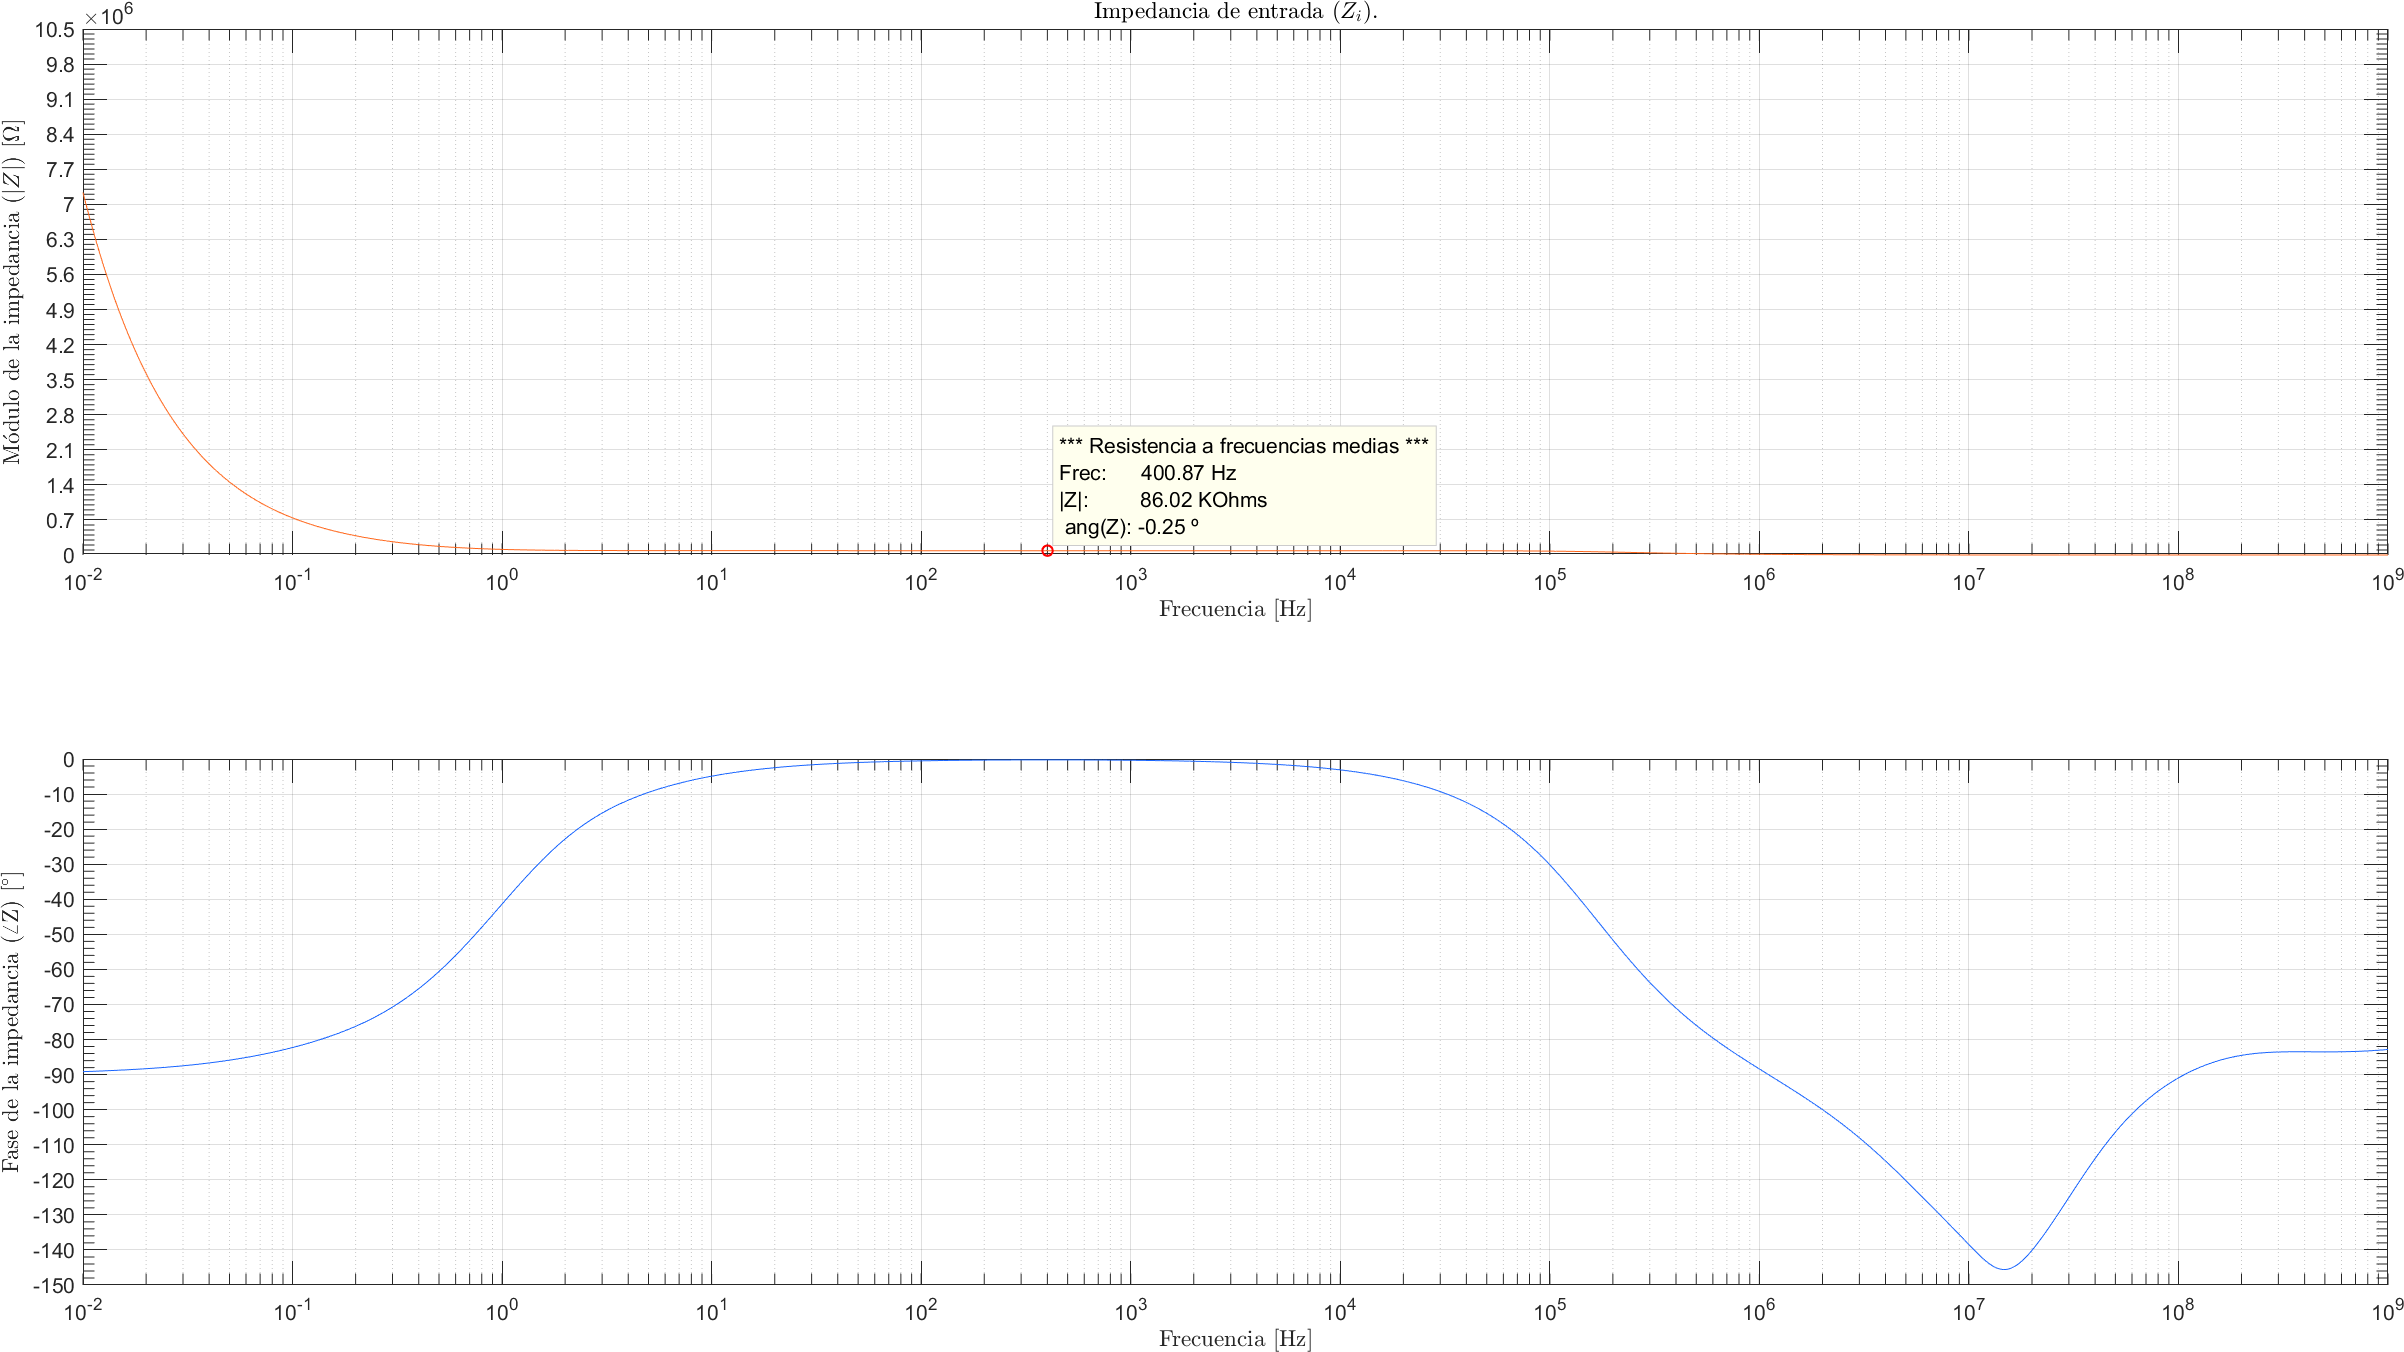
\includegraphics[width=0.9 \textwidth, angle=90]{./img/puntos/P11b_Ri.png}
\caption{\label{fig:fig_simulated_zi}\footnotesize{Impedancia de entrada hallada por simulación.}}
\end{center}
\end{figure}



\clearpage

\subsubsection{Impedancia de salida hallada por simulación}

En la figura~\figref{fig:fig_simulated_zo} se muestra lo obtenido al simular para obtener la impedancia de salida, el valor a frecuencias medias $17.58 \si[per-mode=symbol]{\milli\ohm}$ se aparta un poco del valor calculado en la sección~\sectref{calculated_zo}, se había calculado $29.6 \si[per-mode=symbol]{\milli\ohm}$, pero por lo dicho en dicha sección acerca del cálculo de la impedancia de salida a lazo abierto y por la fuerte dependencia del valor con la ganancia de lazo, que se calcula en forma aproximada, era esperable la diferencia.


\begin{figure}[H] %htb
\begin{center}
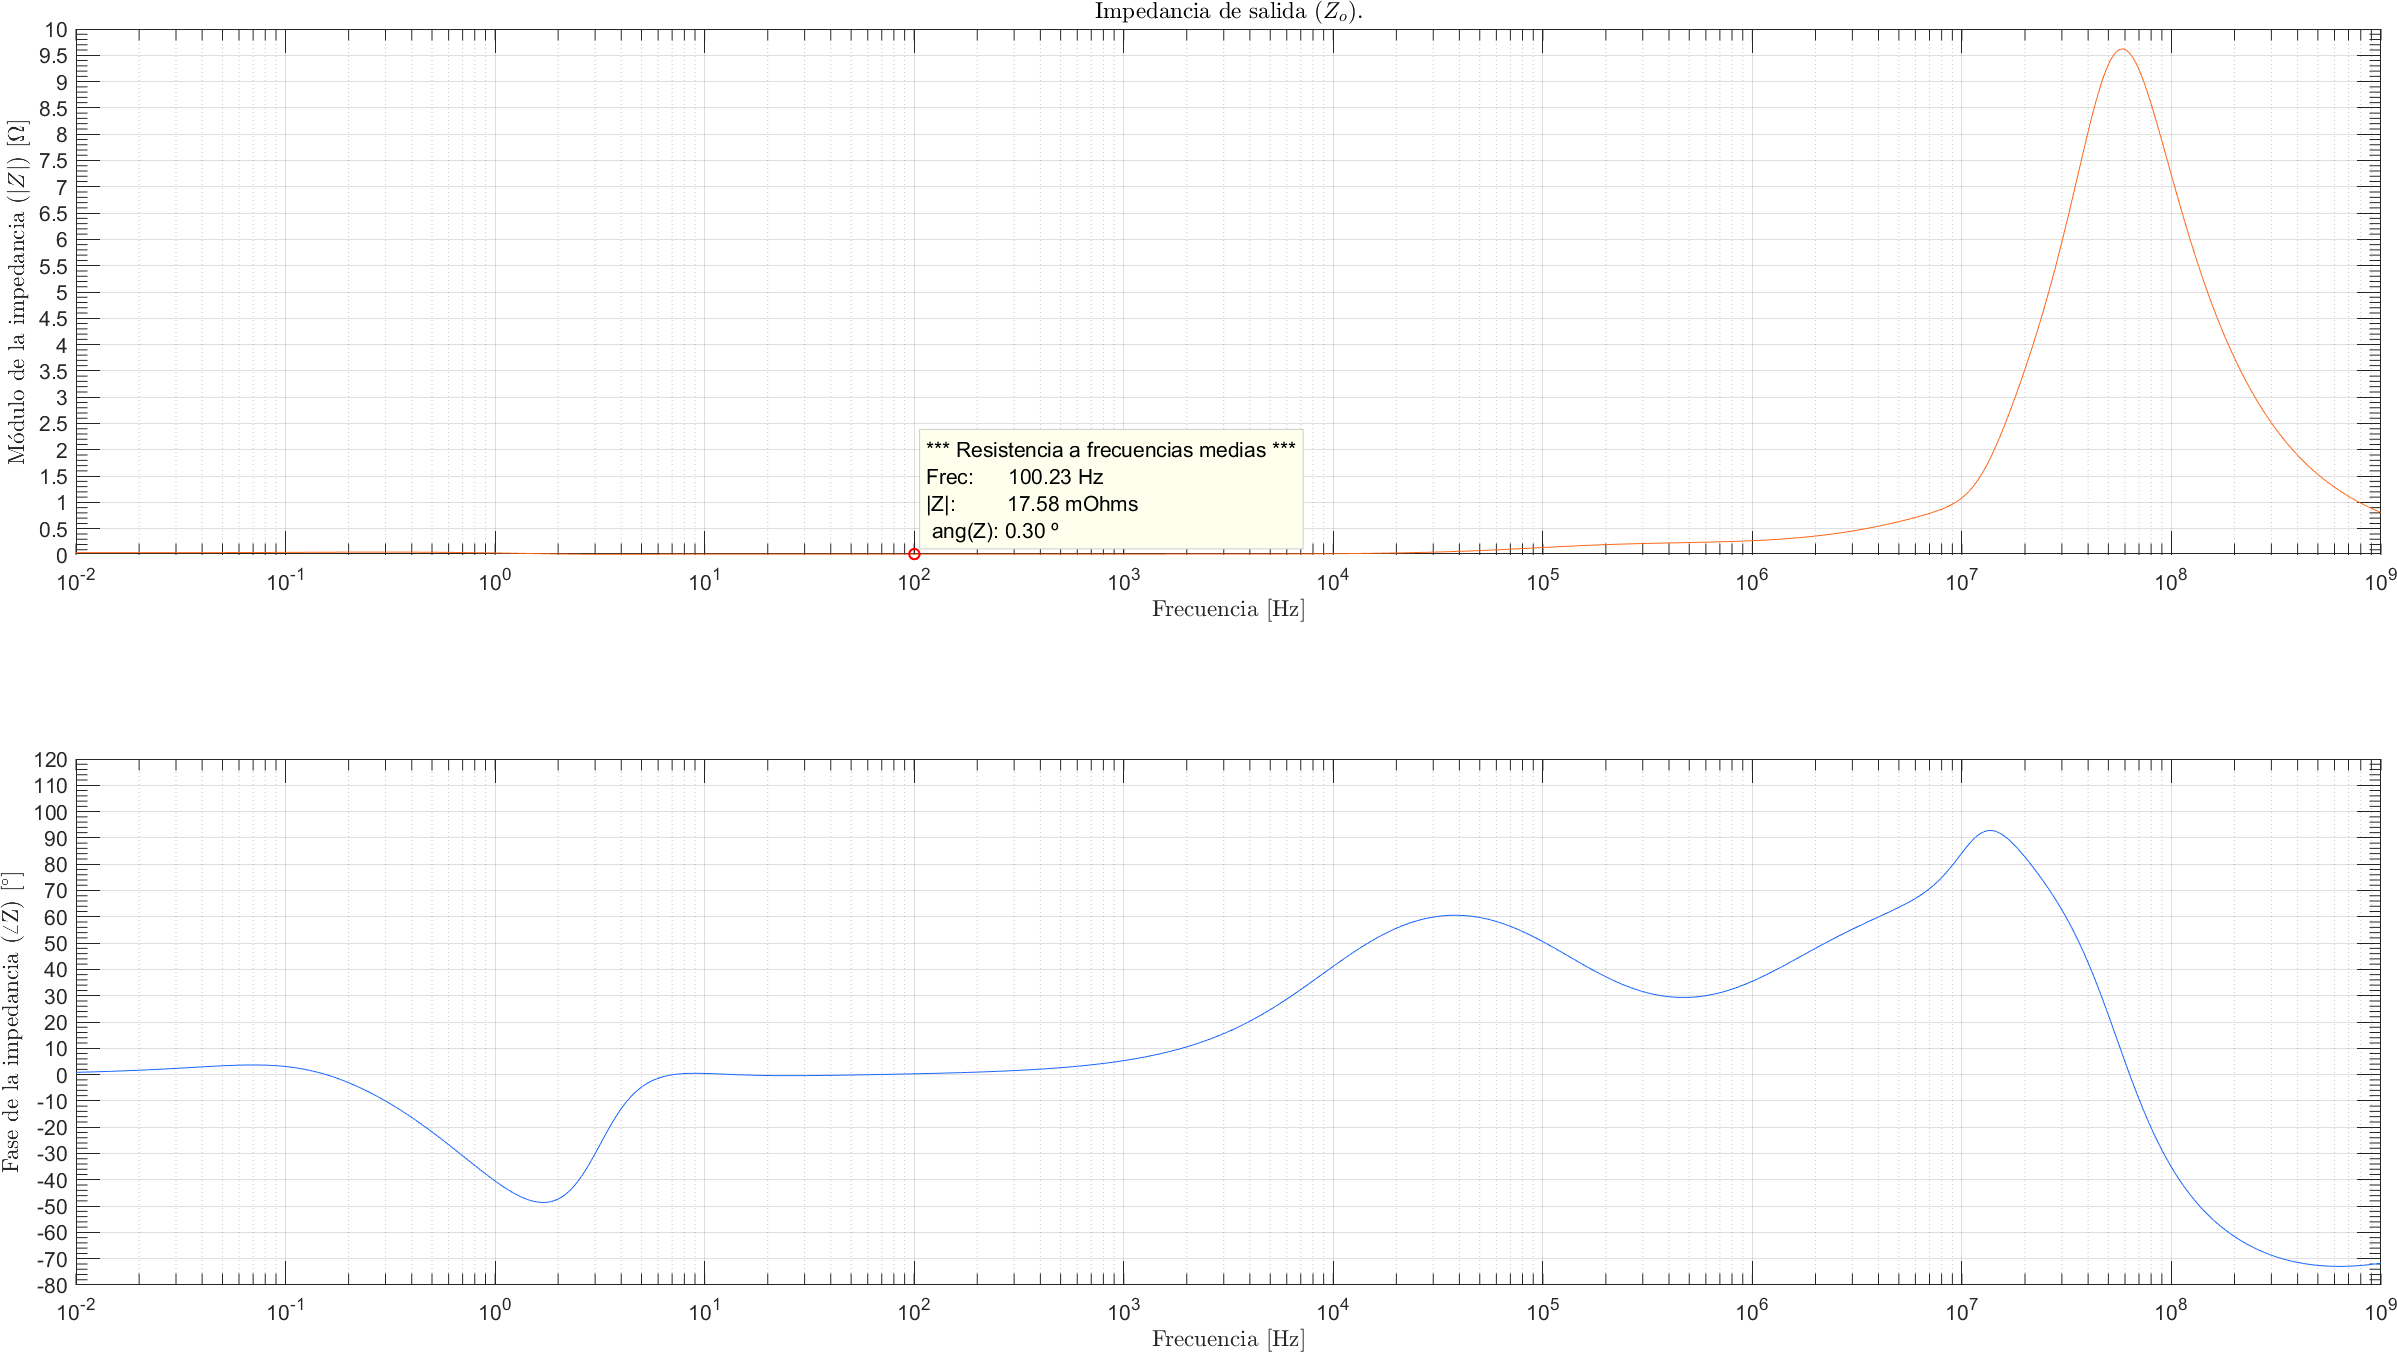
\includegraphics[width=0.9 \textwidth, angle=90]{./img/puntos/P11c_Ro.png}
\caption{\label{fig:fig_simulated_zo}\footnotesize{Impedancia de salida hallada por simulación.}}
\end{center}
\end{figure}



\clearpage

\subsubsection{Respuesta en frecuencia para $1 \si[per-mode=symbol]{\watt}$ sobre la carga}

En la figura~\figref{fig:fig_RF_1W} se muestra lo obtenido al simular para obtener la respuesta en frecuencia a $1 \si[per-mode=symbol]{\watt}$ de potencia sobre la carga, en la misma se puede ver el valor del ancho de banda encontrado, $129.55 \si[per-mode=symbol]{\kilo\hertz}$.

\begin{figure}[H] %htb
\begin{center}
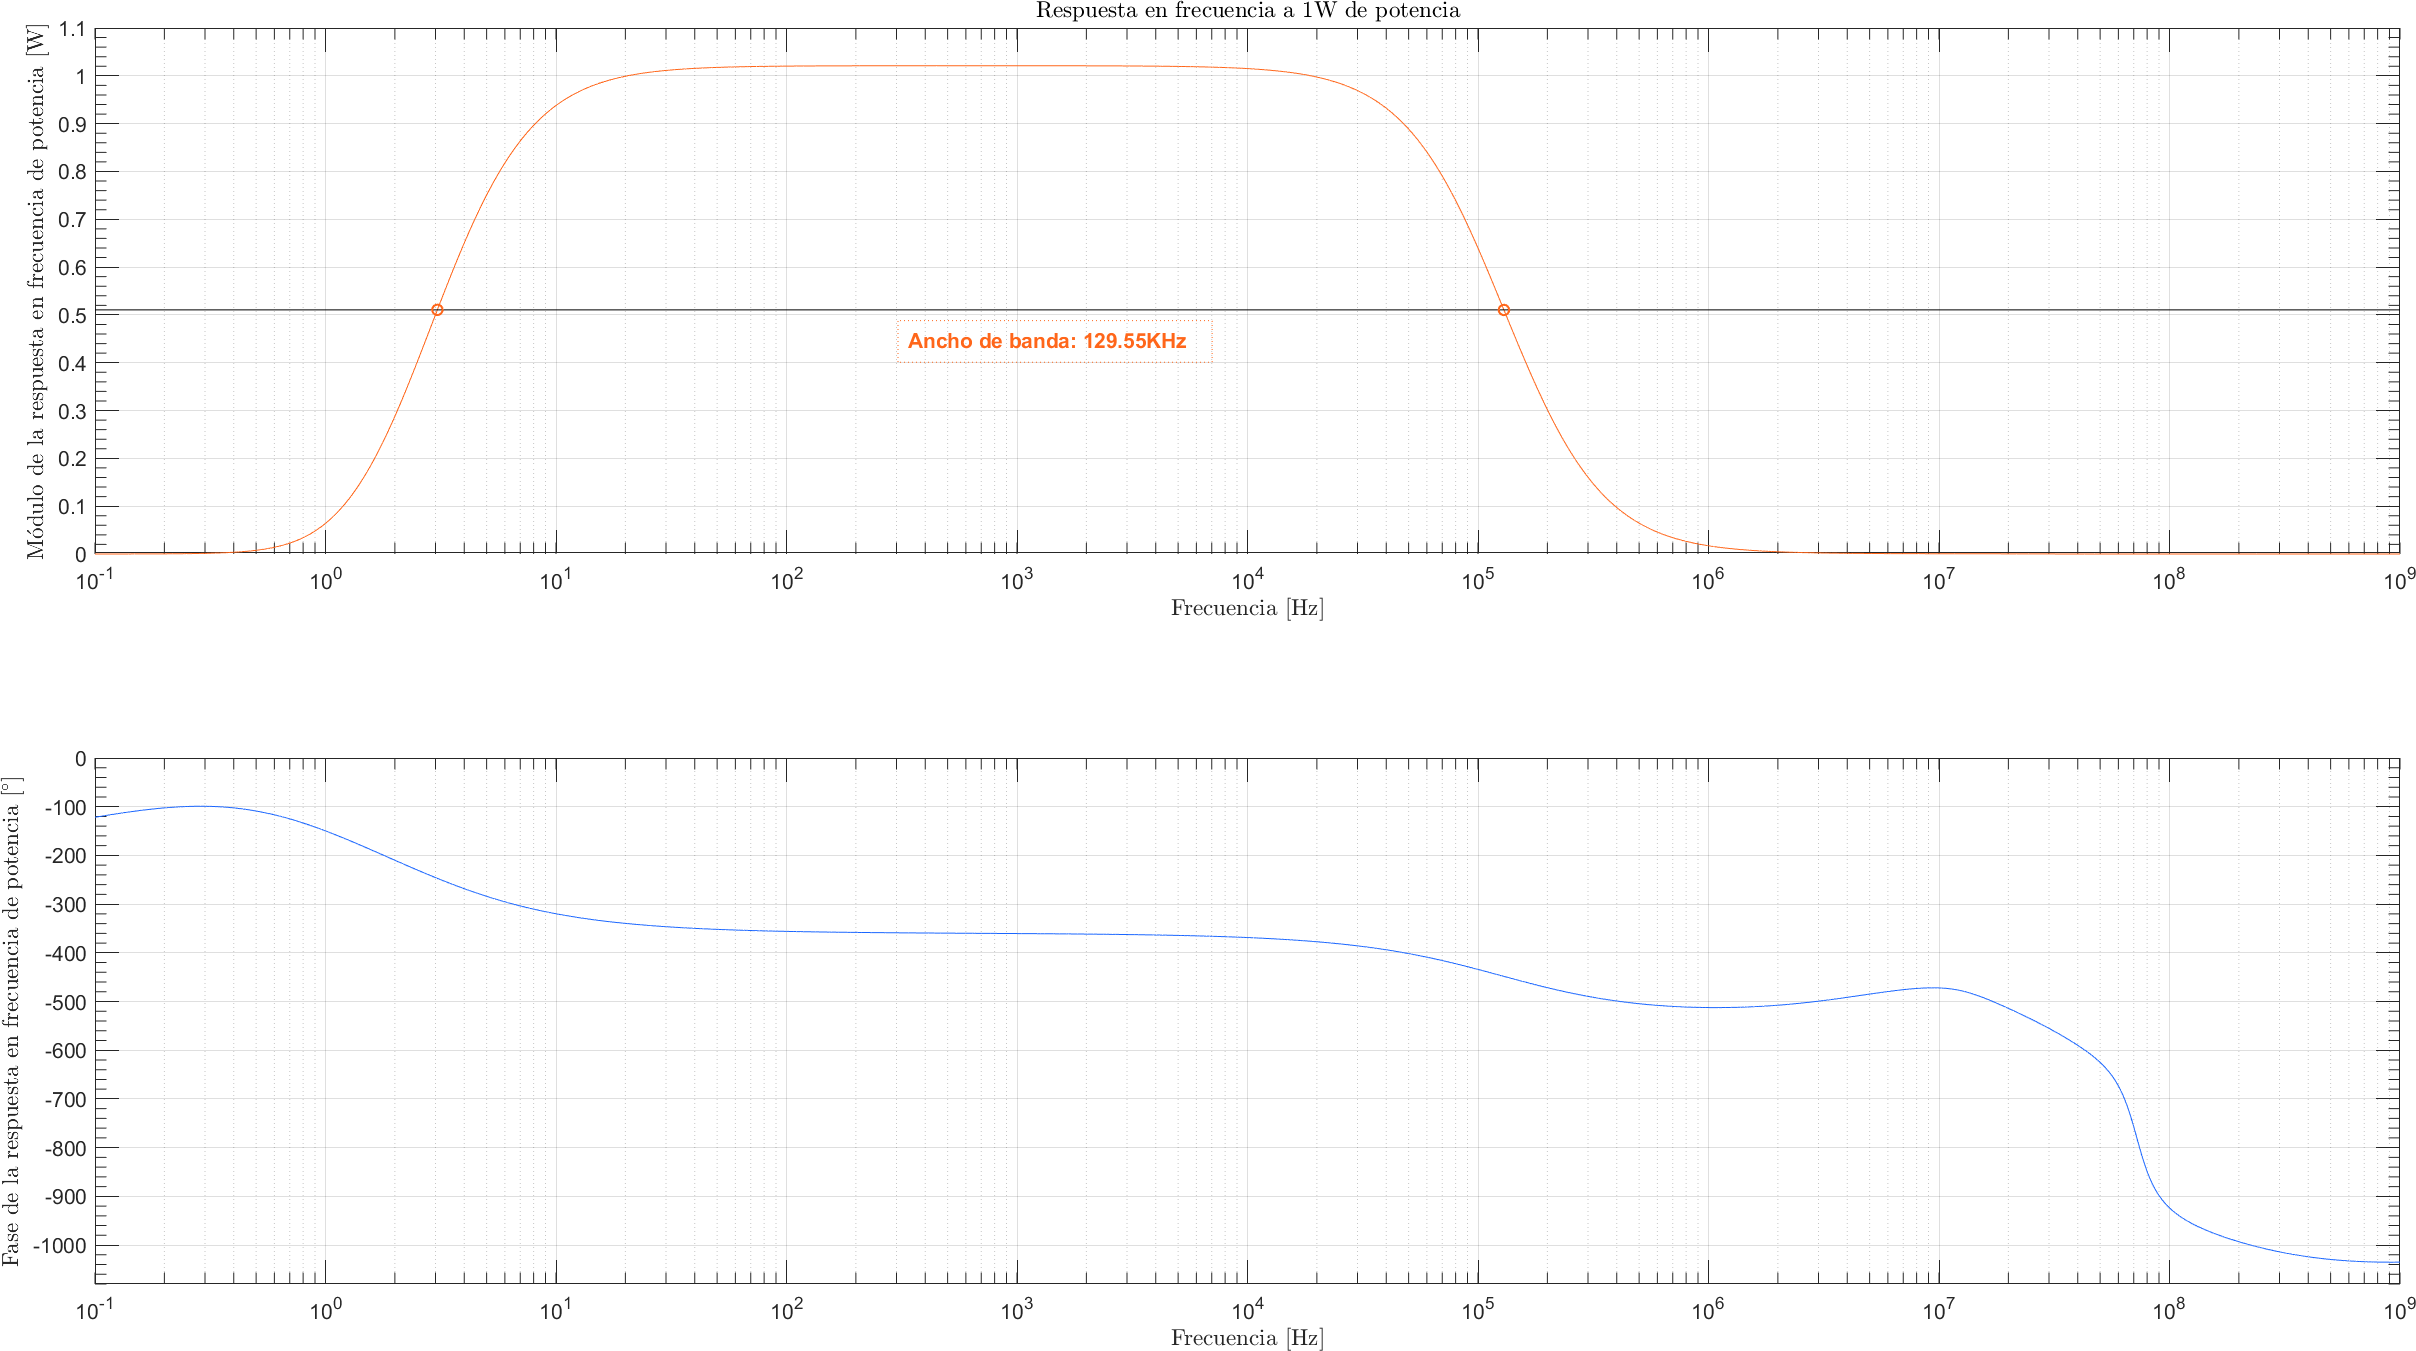
\includegraphics[width=0.9 \textwidth, angle=90]{./img/puntos/P11d_RF_1W.png}
\caption{\label{fig:fig_RF_1W}\footnotesize{Respuesta en frecuencia para $1 \si[per-mode=symbol]{\watt}$ sobre la carga.}}
\end{center}
\end{figure}


\clearpage

\subsubsection{Ancho de banda de potencia, a máxima potencia sobre la carga}

En la figura~\figref{fig:fig_RF_MAX_POWER} se muestra lo obtenido al simular para obtener la respuesta en frecuencia a $1 \si[per-mode=symbol]{\watt}$ de potencia sobre la carga, en la misma se puede ver el valor del ancho de banda encontrado, $129.55 \si[per-mode=symbol]{\kilo\hertz}$, idéntico que para el caso de $1 \si[per-mode=symbol]{\watt}$ .

\begin{figure}[H] %htb
\begin{center}
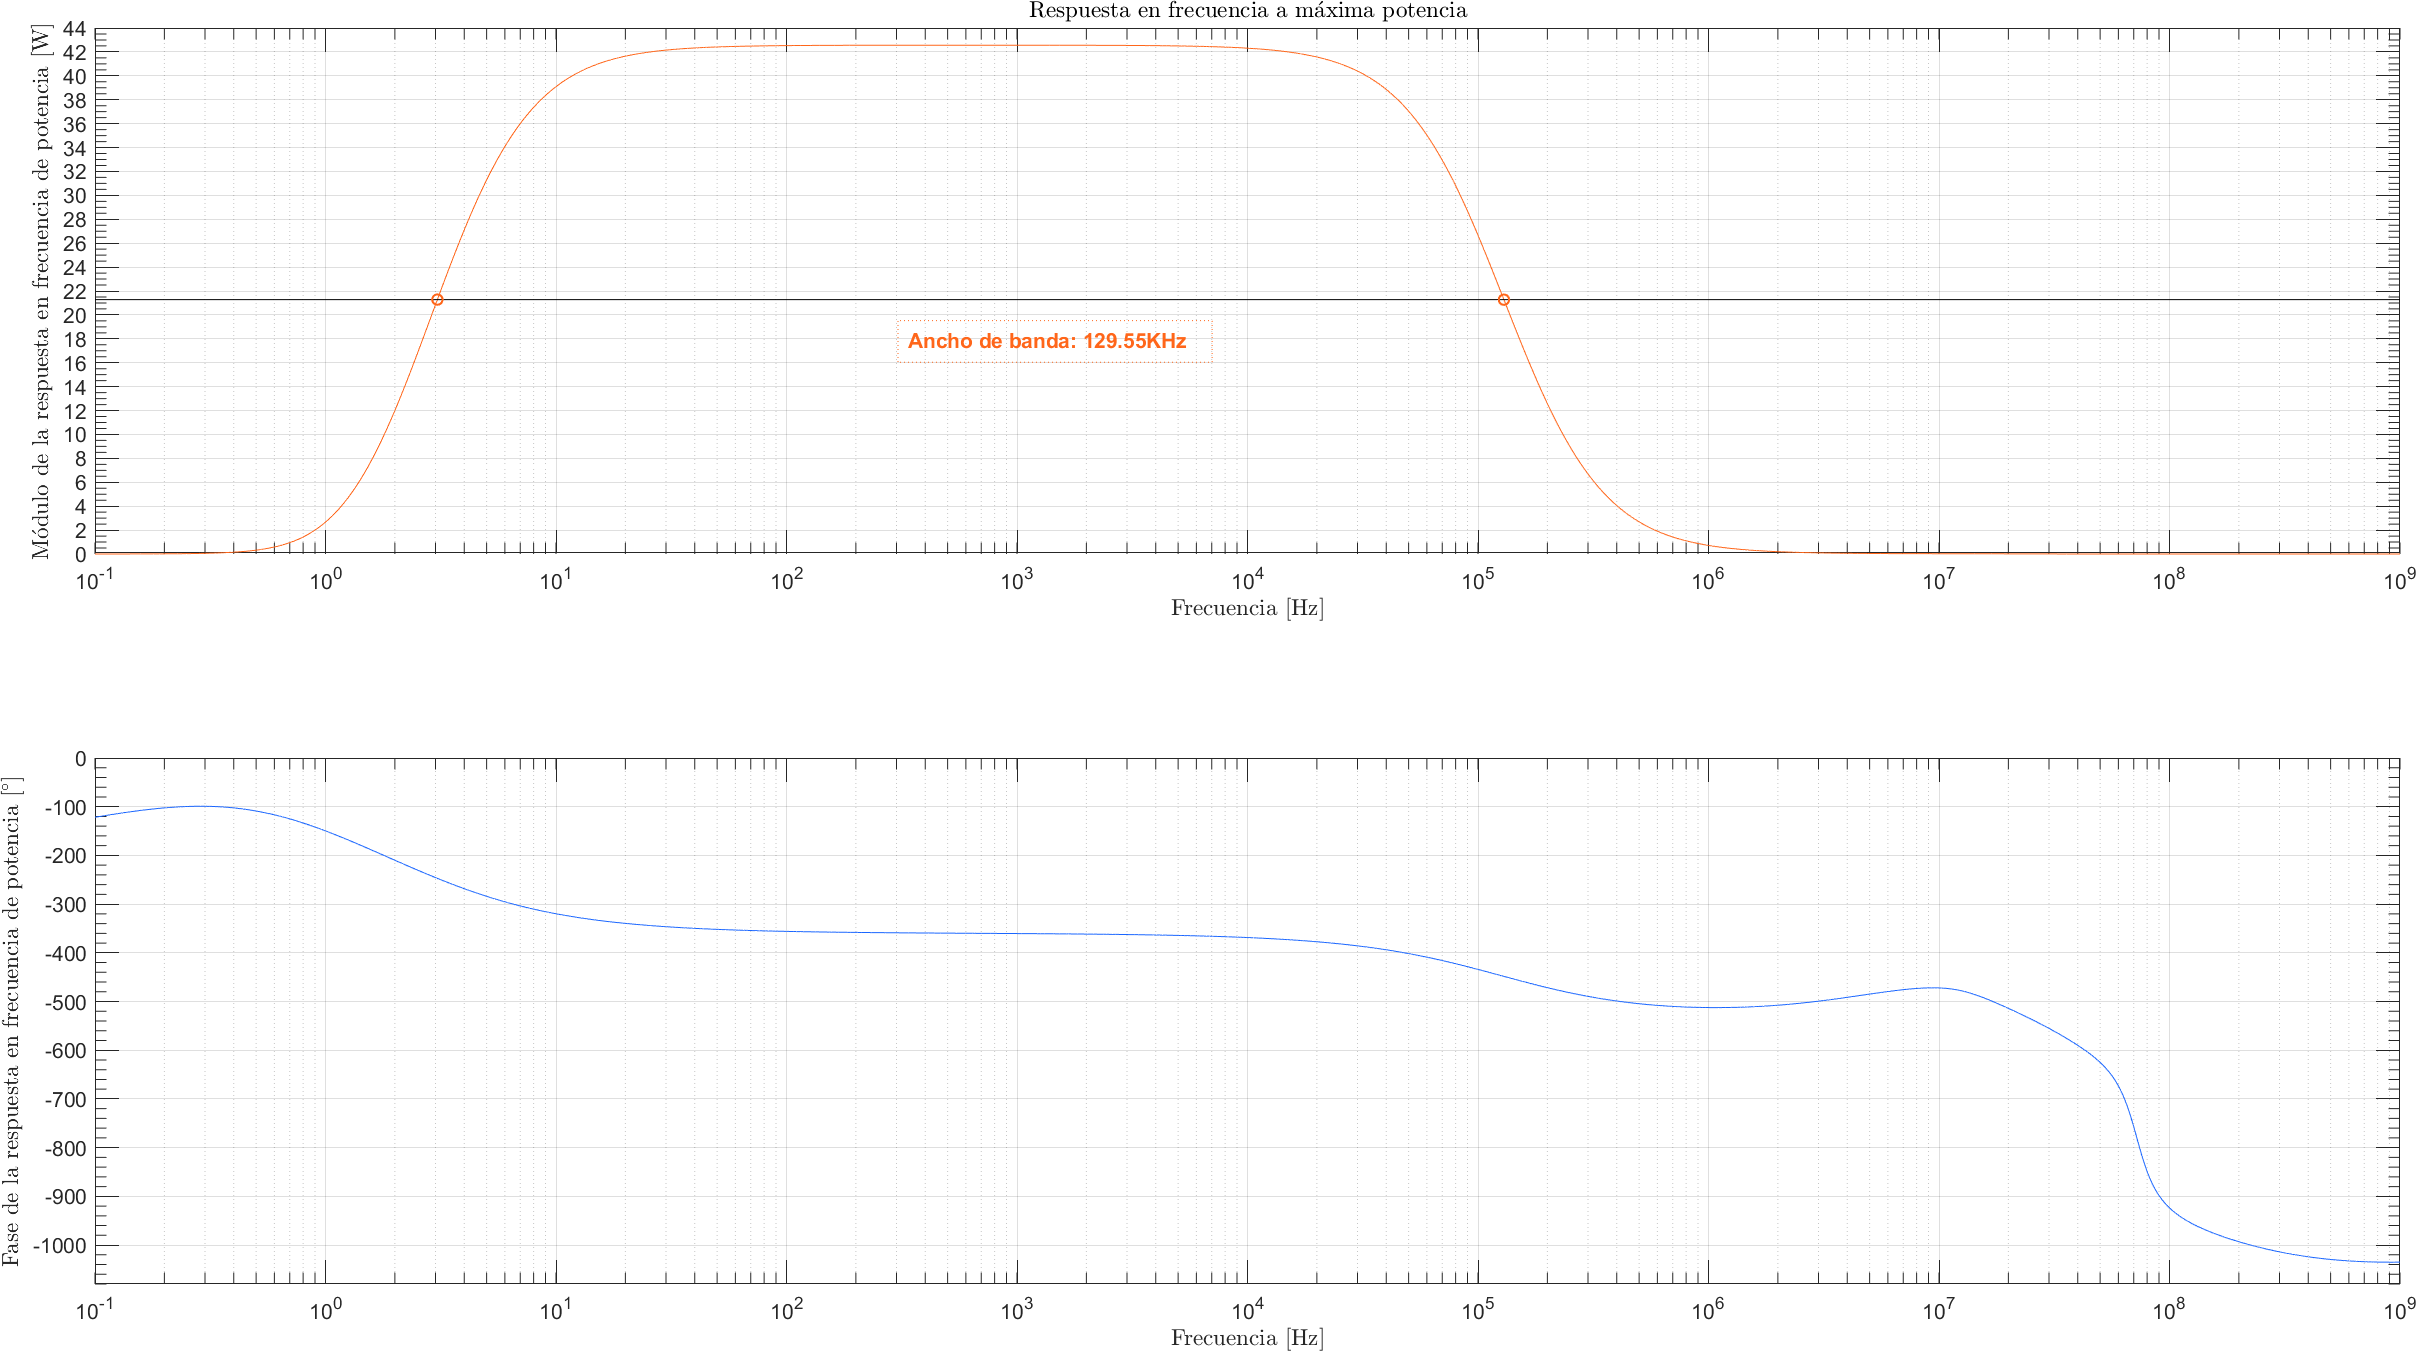
\includegraphics[width=0.9 \textwidth, angle=90]{./img/puntos/P11e_Power_BW.png}
\caption{\label{fig:fig_RF_MAX_POWER}\footnotesize{Respuesta en frecuencia para máxima potencia sobre la carga.}}
\end{center}
\end{figure}


\clearpage

\subsubsection{Respuesta al escalón en pequeña señal}

En la figura~\figref{fig:fig_step_small_signal} se muestra lo obtenido al simular para obtener la respuesta al escalón en pequeña señal, se limitó la salida a un valor de $1 \si[per-mode=symbol]{\volt}$ de pico. La respuesta tiene la forma esperada para un amplificador con acoples capacitivos.

\begin{figure}[H] %htb
\begin{center}
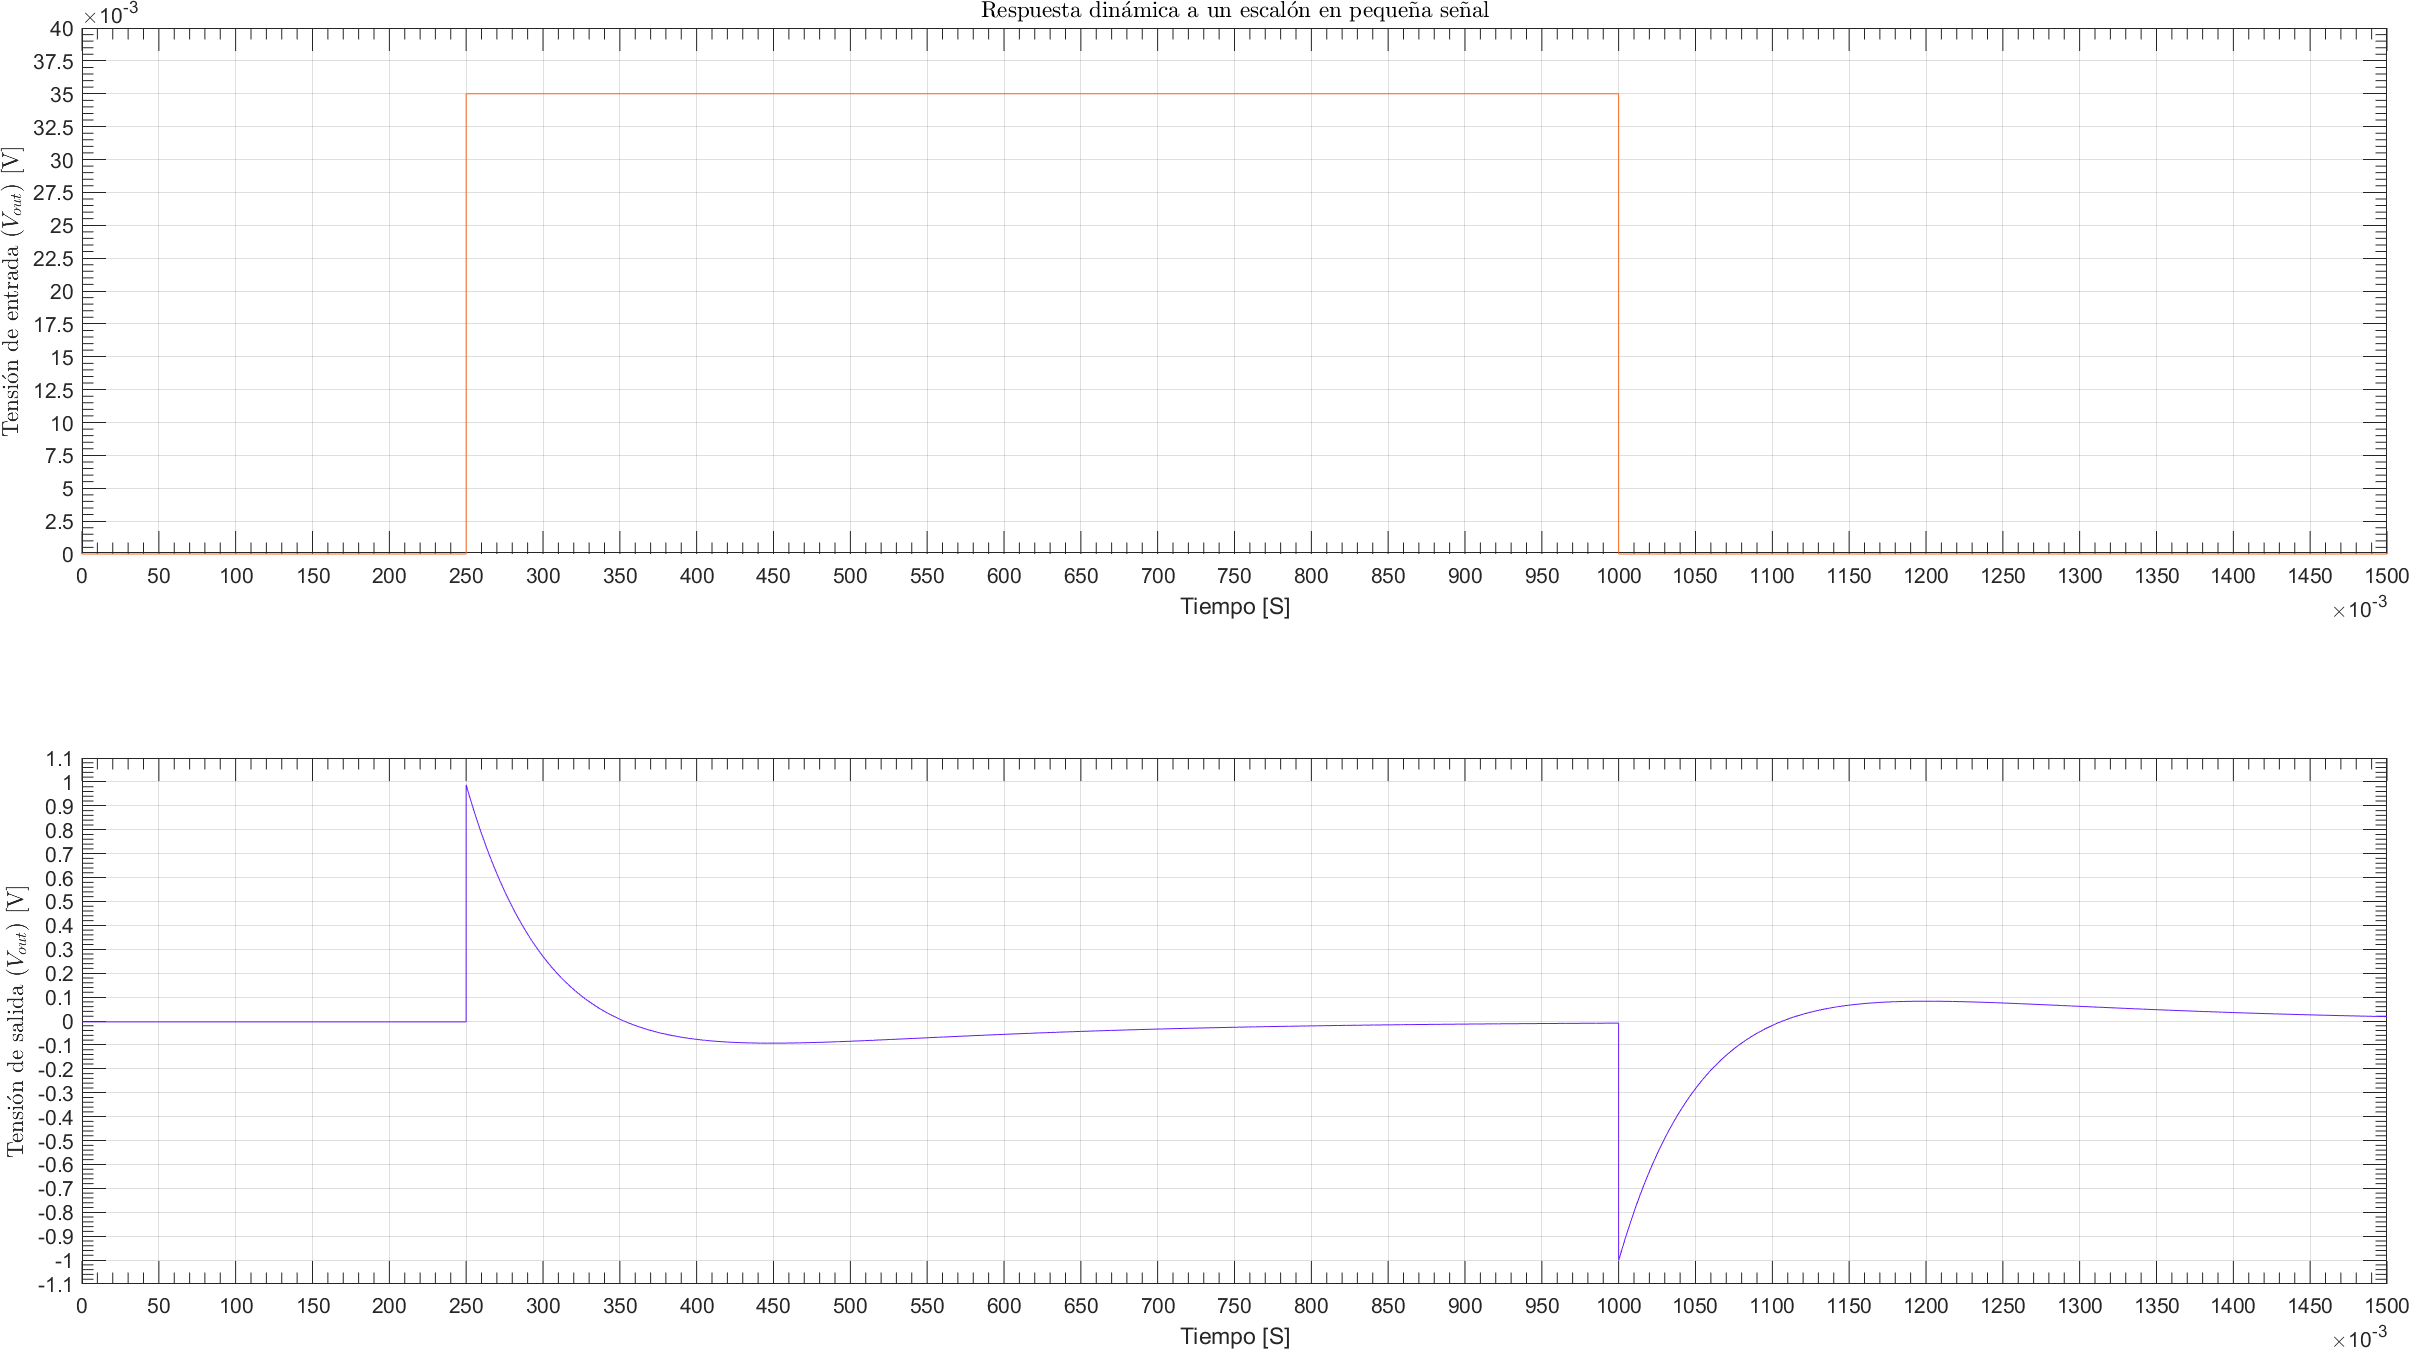
\includegraphics[width=0.9 \textwidth, angle=90]{./img/puntos/P11f_I_step_small_signal.png}
\caption{\label{fig:fig_step_small_signal}\footnotesize{Respuesta al escalón en pequeña señal.}}
\end{center}
\end{figure}


En la figura~\figref{fig:fig_step_small_signal_zoom} se muestra la ampliación del flanco ascendente de la salida, donde se puede apreciar el tiempo de crecimiento, usando la directiva de \textbf{SPICE}, \textit{.measure}, se calculó directamente de la simulación el tiempo de crecimiento entre $10\%$ y $90\%$ y se computó en base a este el ancho de banda del circuito. Se utilizó la expresión que relaciona ancho de banda con el tiempo de crecimiento en un circuito con un solo polo:

\begin{equation}
BW = \frac{0.35}{T_{rise}}
\end{equation}

Se obtuvo:

\begin{equation}
T_{rise} = 2.78 \si[per-mode=symbol]{\micro\second}
\end{equation}


\begin{equation}
\boxed{BW = 125.863 \si[per-mode=symbol]{\kilo\hertz}}
\end{equation}



\begin{figure}[H] %htb
\begin{center}
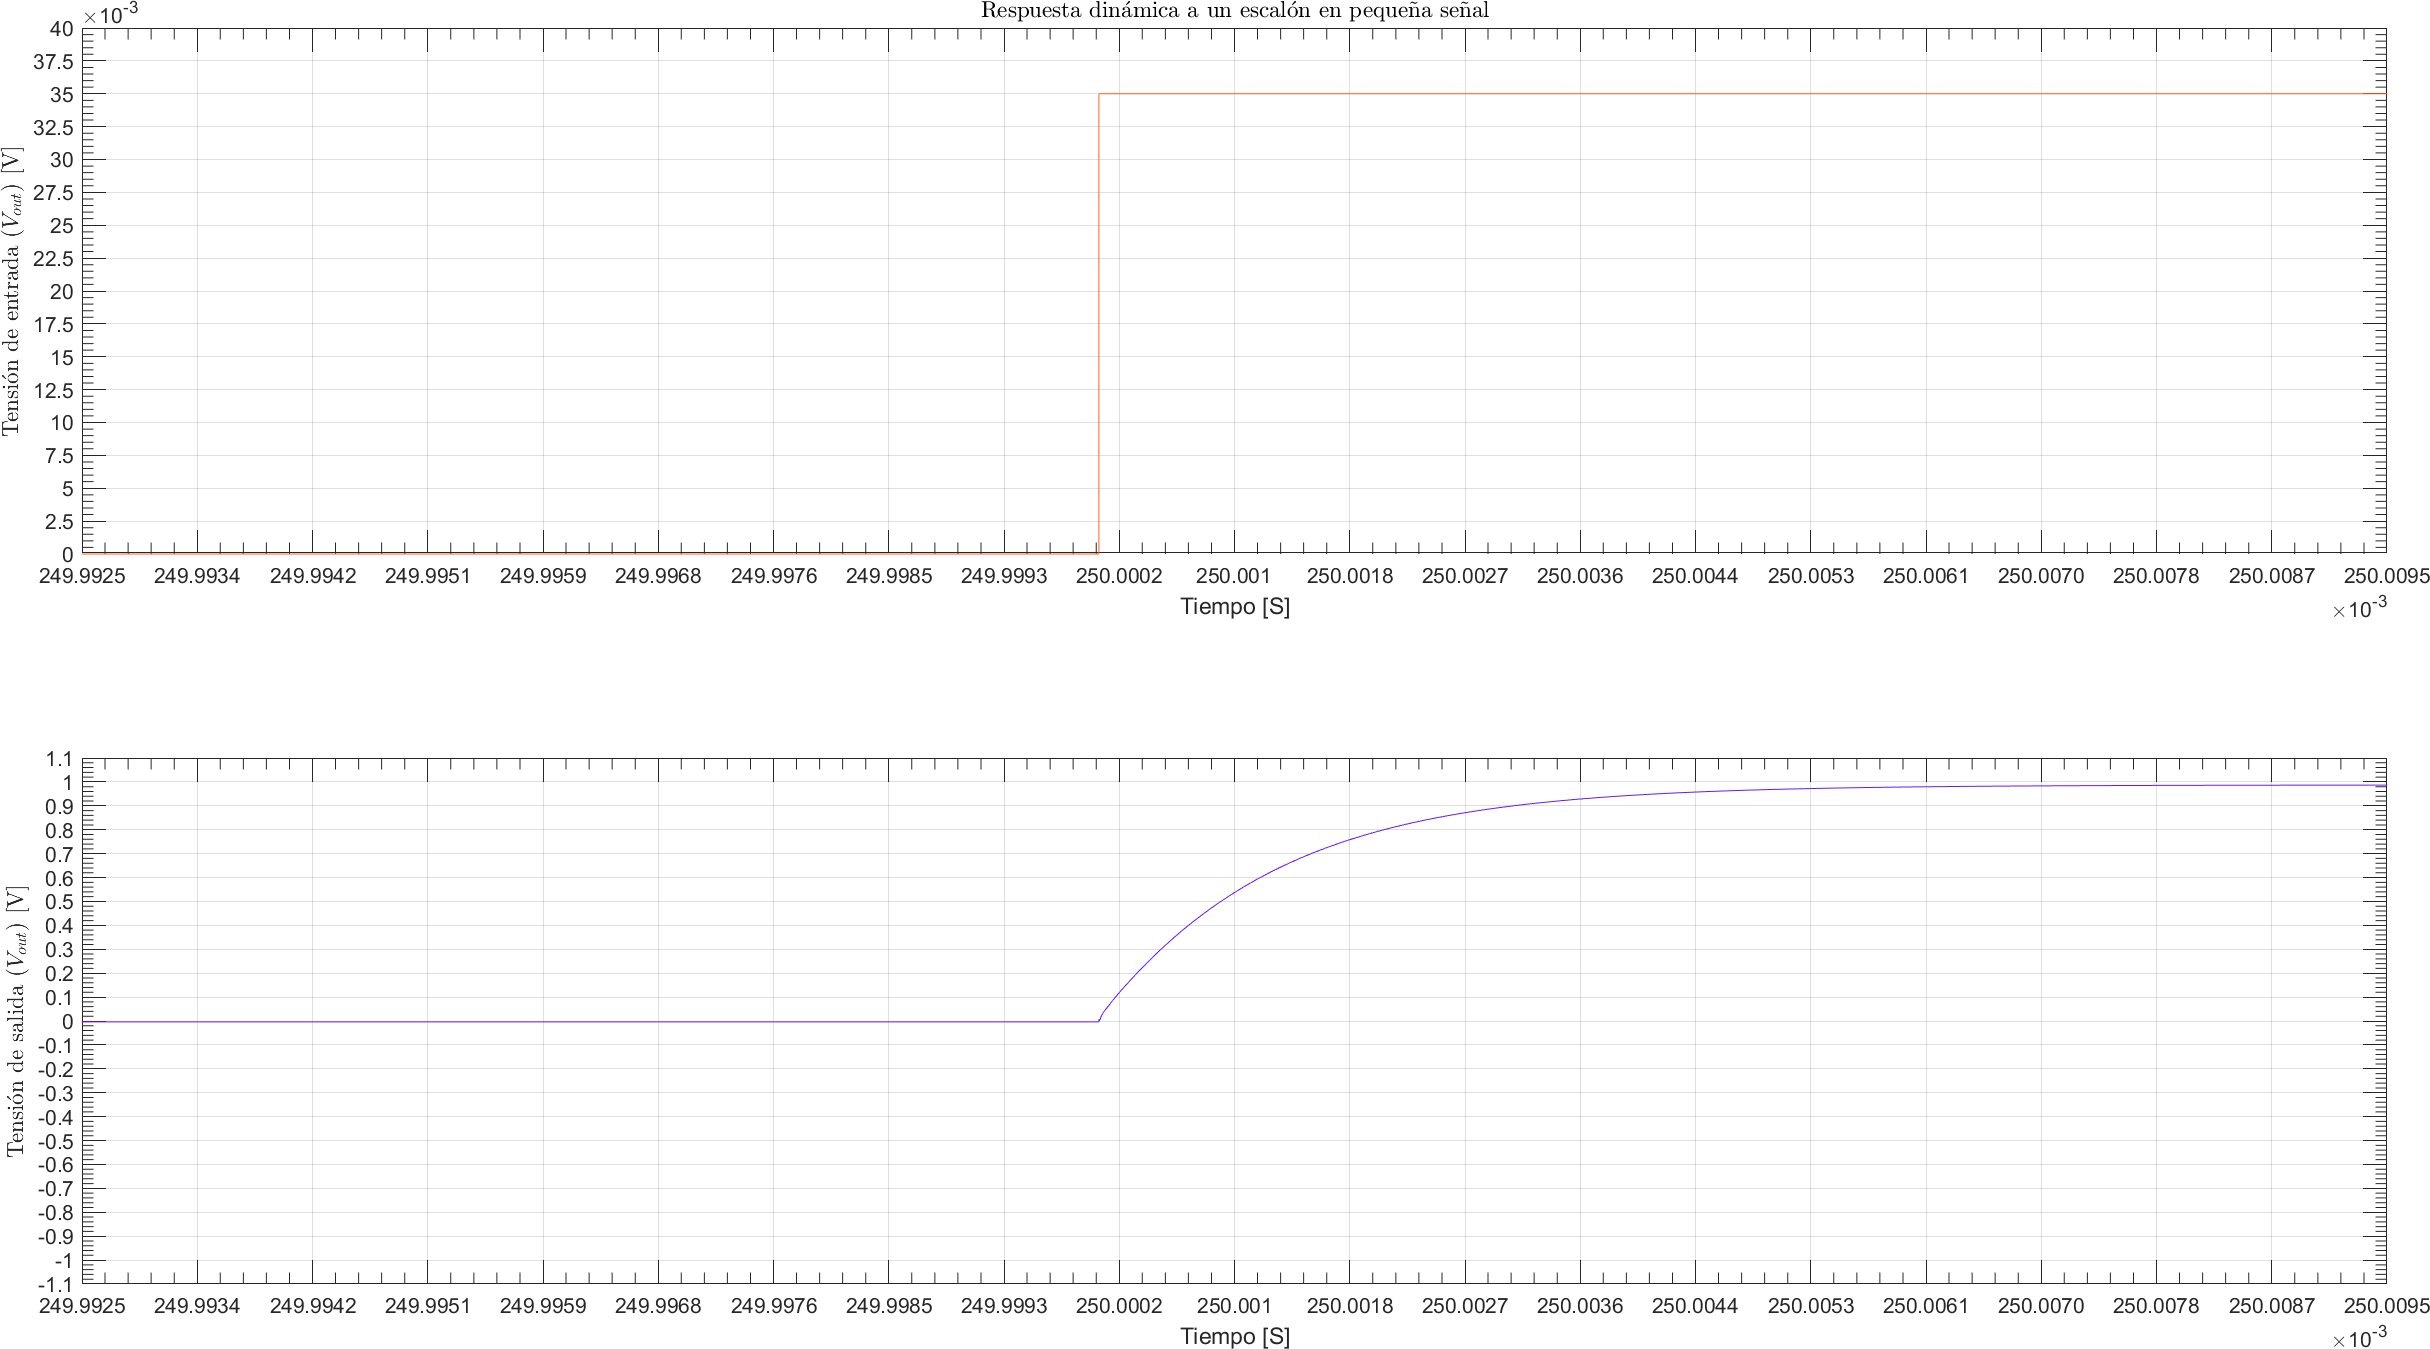
\includegraphics[width=0.9 \textwidth, angle=90]{./img/puntos/P11f_I_step_small_signal_zoom.png}
\caption{\label{fig:fig_step_small_signal_zoom}\footnotesize{Respuesta al escalón en pequeña señal, ampliación del flanco.}}
\end{center}
\end{figure}

\clearpage

\subsubsection{Respuesta al escalón en gran señal}

En la figura~\figref{fig:fig_step_big_signal} se muestra lo obtenido al simular para obtener la respuesta al escalón en gran señal, se llevó la salida a un valor cercano al máximo sin distorsión.

\begin{figure}[H] %htb
\begin{center}
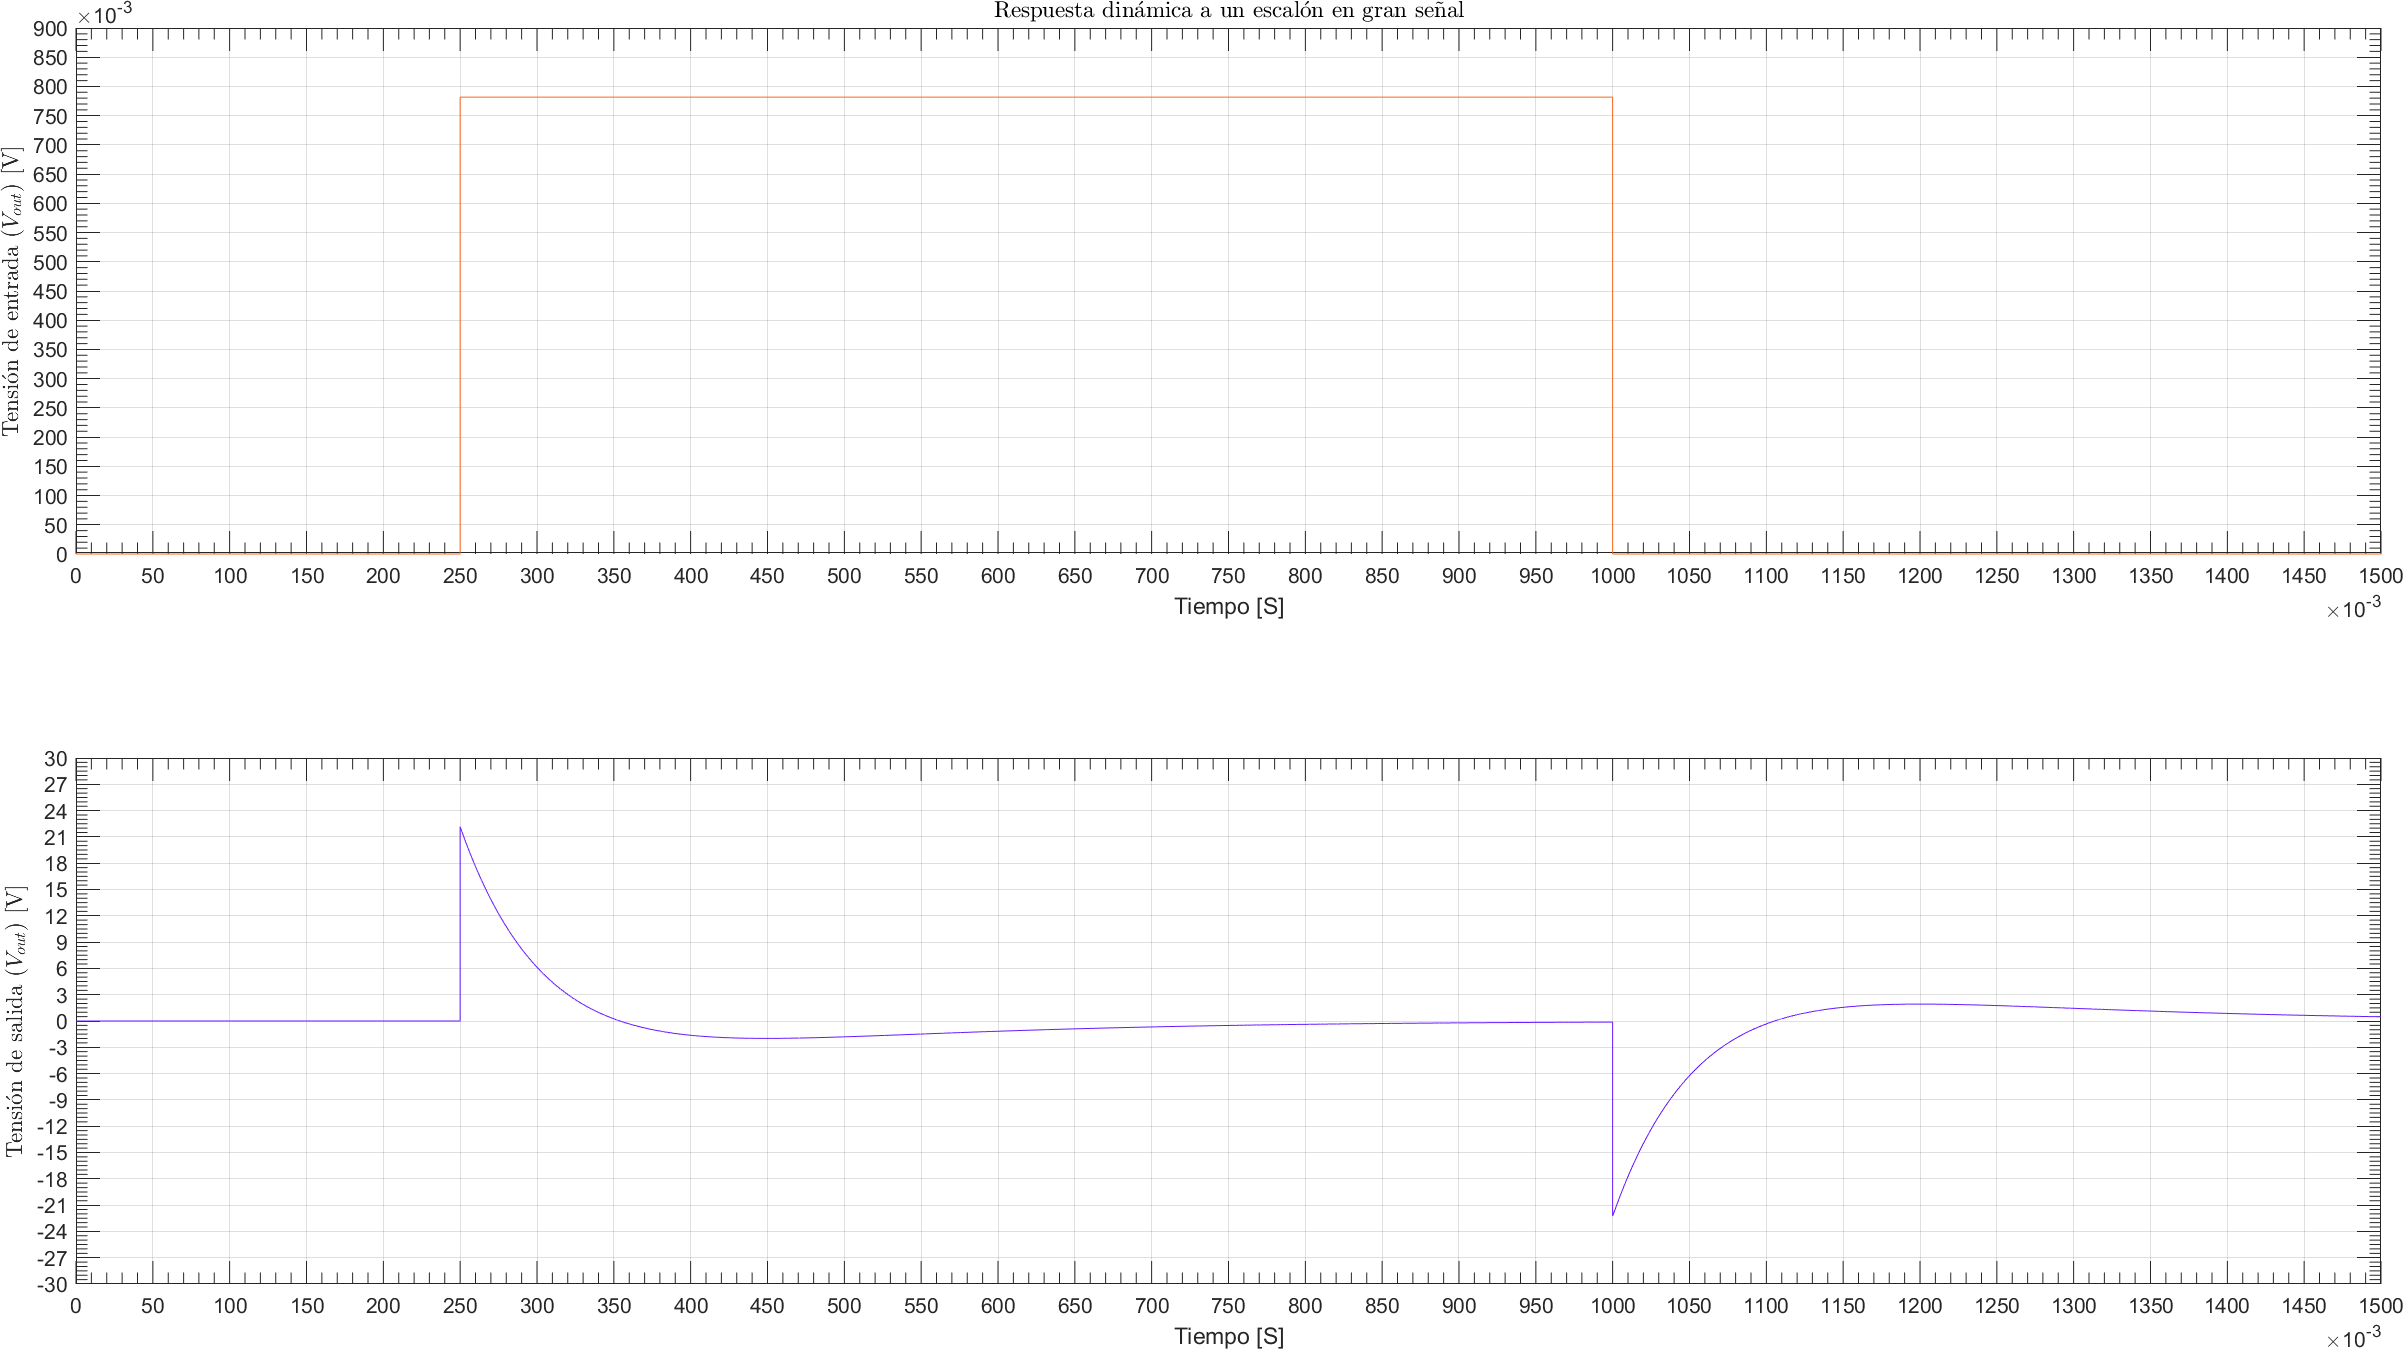
\includegraphics[width=0.9 \textwidth, angle=90]{./img/puntos/P11f_I_step_big_signal.png}
\caption{\label{fig:fig_step_big_signal}\footnotesize{Respuesta al escalón en gran señal.}}
\end{center}
\end{figure}


En la figura~\figref{fig:fig_step_big_signal_zoom} se muestra la ampliación del flanco ascendente de la salida, donde se puede apreciar el tiempo de crecimiento, usando la directiva de \textbf{SPICE}, \textit{.measure}, se calculó directamente de la simulación el \textbf{\quotemarks{slew~rate}}, como la pendiente de subida en el flanco ascendente, se obtuvo:


\begin{equation}
\boxed{SR = 4.39 \si[per-mode=symbol]{\volt\per\micro\second}}
\end{equation}



\begin{figure}[H] %htb
\begin{center}
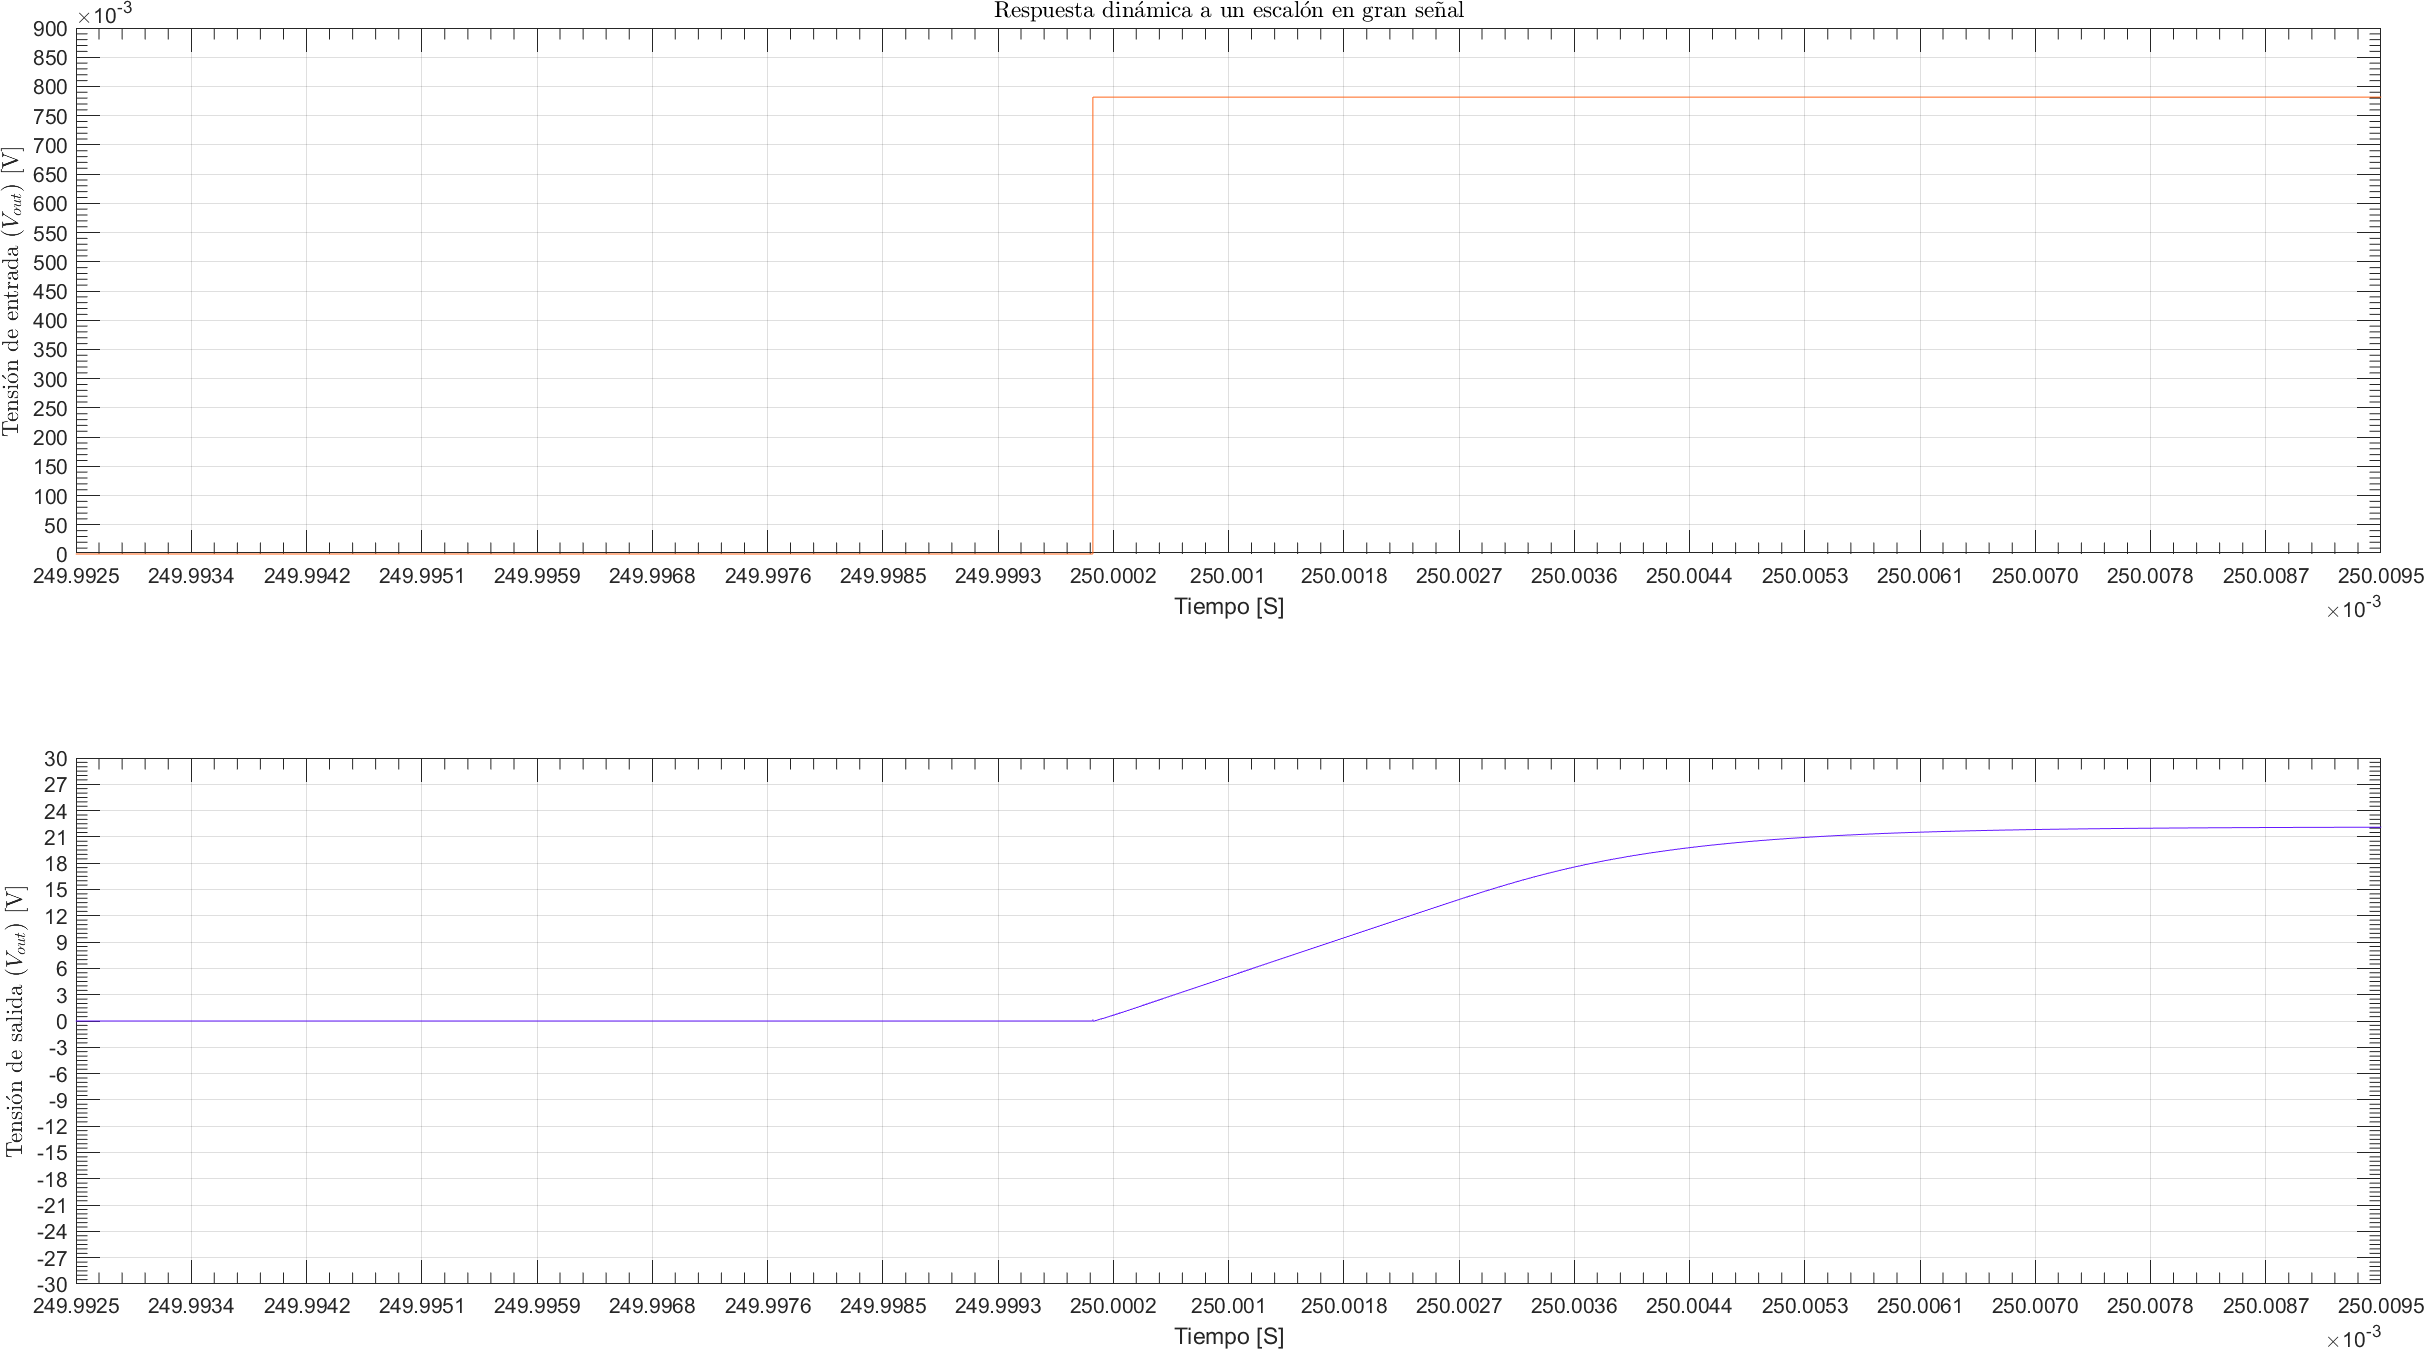
\includegraphics[width=0.9 \textwidth, angle=90]{./img/puntos/P11f_I_step_big_signal_zoom.png}
\caption{\label{fig:fig_step_big_signal_zoom}\footnotesize{Respuesta al escalón en gran señal, ampliación del flanco.}}
\end{center}
\end{figure}

\clearpage


\subsubsection{Margen de fase del amplificador}

En la figura~\figref{fig:fig_phase_margin} se muestra lo obtenido al simular para obtener el margen de fase del circuito, para esta simulación se abrió el lazo de realimentación para la señal y se tomó la respuesta de la cascada del amplificador con la realimentación, en la figura~\figref{fig:fig_loop_gain_circuit}, se puede ver el circuito utilizado para esta simulación. El valor obtenido para el margen de fase es:

\begin{equation}
\boxed{PM = 113.72 \si[per-mode=symbol]{\degree}}
\end{equation}

\begin{figure}[H] %htb
\begin{center}
\includegraphics[width=0.9 \textwidth, angle=90]{./img/puntos/P11g_phase_margin.png}
\caption{\label{fig:fig_phase_margin}\footnotesize{Margen de fase.}}
\end{center}
\end{figure}

\begin{figure}[H] %htb
\begin{center}
\includegraphics[width=0.9 \textwidth, angle=90]{./img/circuitos_usados/P11g_phase_margin.png}
\caption{\label{fig:fig_loop_gain_circuit}\footnotesize{Circuito usado para simular la ganancia de lazo.}}
\end{center}
\end{figure}

\clearpage

\subsubsection{Distorsión armónica del amplificador}

En el cuadro~\tableref{table:table_THD} se resumen los resultados obtenidos al realizar la simulación para determinar la distorsión armónica total (\textbf{THD}) para 8 combinaciones de frecuencia y potencia de salida sobre la carga. El cálculo se realizo directamente con el comando \textbf{SPICE} \textit{.fourier}, teniendo en cuenta nueve armónicas de la señal y usando todos los datos de aproximadamente $1\si[per-mode=symbol]{\second}$ de simulación.



%% \noindent
%% \begin{center}
 
%%\begin{spacing}{1}  
\begin{table}[H]  %%\centering
    
    \setlength\arrayrulewidth{1.5pt}
    \arrayrulecolor{white}
    \def\clinecolor{\hhline{|>{\arrayrulecolor{white}}-%
    >{\arrayrulecolor{white}}|-|-|-|-|}}
\resizebox{0.8 \textwidth}{!}{% 
       
\begin{tabularx}{1 \textwidth}%
    {|
    >{\columncolor{white} \centering\arraybackslash}m{0.32\linewidth}
     |
    >{\columncolor{white} \centering\arraybackslash}m{0.17\linewidth}
     |
    >{\columncolor{white} \centering\arraybackslash}m{0.17\linewidth}
     |
    >{\columncolor{white} \centering\arraybackslash}m{0.17\linewidth}
     |
    >{\columncolor{white} \centering\arraybackslash}m{0.17\linewidth}
     |
    }
    \rowcolor{HeadersColor} \cellcolor{white} \thead{}  & \thead{$0.1 \si[per-mode=symbol]{\watt}$} & \thead{$1 \si[per-mode=symbol]{\watt}$} & \thead{$10 \si[per-mode=symbol]{\watt}$} & \thead{$90 \%$ de max.} \\    
    \hhline{|-|-|-|-|}
    \rowcolor{gray!20} \cellcolor{HeadersColor} \color{white} $1 \si[per-mode=symbol]{\kilo\hertz}$ & $0.055\%$ & $0.023\%$ & $0.014\%$ & $0.055\%$  \\
    \hhline{|-|-|-|-|}
    \rowcolor{gray!20} \cellcolor{HeadersColor} \color{white} $10 \si[per-mode=symbol]{\kilo\hertz}$ & $0.144\%$ & $0.077\%$ & $0.057\%$ & $0.107\%$   \\
    \hhline{|-|-|-|-|}       
    \end{tabularx}}
	\caption{\footnotesize{Distorsión armónica total (\textbf{THD}).}}
	\label{table:table_THD}
\end{table}
%%\end{spacing}

%% \end{center}

Vemos que la distorsión es menor para $1 \si[per-mode=symbol]{\kilo\hertz}$  de frecuencia de entrada y también que presenta un mínimo alrededor de las potencias medias, es decir, disminuye de bajas a medias potencias y sube de medias a altas potencias.


\clearpage

\subsubsection{Distorsión por intermodulación del amplificador}

En el cuadro~\tableref{table:table_IMD} se resumen los resultados obtenidos al realizar la simulación para determinar la distorsión por intermodulación (\textbf{IMD}) para 4 potencias de salida sobre la carga. El cálculo se realizo con el comando \textbf{SPICE} \textit{.fourier}, se tomaron las armónicas de $100 \si[per-mode=symbol]{\hertz}$ hasta la armónica $55$, de modo de tomar $5$ armónicas por arriba y $5$ armónicas por debajo del tono puro de $5 \si[per-mode=symbol]{\kilo\hertz}$ , y usando todos los datos de aproximadamente $1\si[per-mode=symbol]{\second}$ de simulación.\\
Se observa que la \textbf{IMD} parece crecer para valores bajos y altos de la potencia de salida, teniendo un mínimo a potencias medias.



%% \noindent
%% \begin{center}
 
%%\begin{spacing}{1}  
\begin{table}[H]  %%\centering
    
    \setlength\arrayrulewidth{1.5pt}
    \arrayrulecolor{white}
    \def\clinecolor{\hhline{|>{\arrayrulecolor{white}}-%
    >{\arrayrulecolor{white}}|-|-|-|-|}}
\resizebox{0.8 \textwidth}{!}{% 
       
\begin{tabularx}{1 \textwidth}%
    {|
    >{\columncolor{white} \centering\arraybackslash}m{0.32\linewidth}
     |
    >{\columncolor{white} \centering\arraybackslash}m{0.17\linewidth}
     |
    >{\columncolor{white} \centering\arraybackslash}m{0.17\linewidth}
     |
    >{\columncolor{white} \centering\arraybackslash}m{0.17\linewidth}
     |
    >{\columncolor{white} \centering\arraybackslash}m{0.17\linewidth}
     |
    }
    \rowcolor{HeadersColor} \cellcolor{white} \thead{}  & \thead{$0.1 \si[per-mode=symbol]{\watt}$} & \thead{$1 \si[per-mode=symbol]{\watt}$} & \thead{$10 \si[per-mode=symbol]{\watt}$} & \thead{$90 \%$ de max.} \\    
    \hhline{|-|-|-|-|}
    \rowcolor{gray!20} \cellcolor{HeadersColor} \color{white} \textbf{IMD} & $0.108 \%$ & $0.043 \%$ & $0.048 \%$ & $0.51 \%$ \\
    \hhline{|-|-|-|-|}     
    \end{tabularx}}
	\caption{\footnotesize{Distorsión armónica total (\textbf{IMD}).}}
	\label{table:table_IMD}
\end{table}
%%\end{spacing}

%% \end{center}



\clearpage

\subsubsection{Rechazo de Ruido de la Fuente de Alimentación (\textbf{\quotemarks{PSNR}}).}

En el cuadro~\tableref{table:table_PSNR} se resumen los resultados obtenidos al realizar la simulación para determinar el rechazo de ruido de la fuente de alimentación (\textbf{PSNR}) para 4 frecuencias de la señal de ruido presente en la fuente de alimentación y para una tensión de pico de ruido de $1 \si[per-mode=symbol]{\milli\volt}$.



%% \noindent
%% \begin{center}
 
%%\begin{spacing}{1}  
\begin{table}[H]  %%\centering
    
    \setlength\arrayrulewidth{1.5pt}
    \arrayrulecolor{white}
    \def\clinecolor{\hhline{|>{\arrayrulecolor{white}}-%
    >{\arrayrulecolor{white}}|-|-|-|-|-|-|}}
\resizebox{0.8 \textwidth}{!}{% 
       
\begin{tabularx}{1 \textwidth}%
    {|
    >{\columncolor{white} \centering\arraybackslash}m{0.25\linewidth}
     |
    >{\columncolor{white} \centering\arraybackslash}m{0.125\linewidth}
     |
    >{\columncolor{white} \centering\arraybackslash}m{0.125\linewidth}
     |
    >{\columncolor{white} \centering\arraybackslash}m{0.125\linewidth}
     |
    >{\columncolor{white} \centering\arraybackslash}m{0.125\linewidth}
     |
    >{\columncolor{white} \centering\arraybackslash}m{0.125\linewidth}
     |
    >{\columncolor{white} \centering\arraybackslash}m{0.125\linewidth}
     |
    }
    \rowcolor{HeadersColor} \cellcolor{white} \thead{}  & \thead{$50 \si[per-mode=symbol]{\hertz}$} & \thead{$100 \si[per-mode=symbol]{\hertz}$} & \thead{$1 \si[per-mode=symbol]{\kilo\hertz}$} & \thead{ $10 \si[per-mode=symbol]{\kilo\hertz}$} & \thead{$50 \si[per-mode=symbol]{\kilo\hertz}$} & \thead{$100 \si[per-mode=symbol]{\kilo\hertz}$}\\    
    \hhline{|-|-|-|-|-|-|}
    \rowcolor{gray!20} \cellcolor{HeadersColor} \color{white} \textbf{PSNR} & $ 53.2 \si[per-mode=symbol]{\decibel} $ & $ 59.1 \si[per-mode=symbol]{\decibel} $ & $ 78.99 \si[per-mode=symbol]{\decibel} $ & $ 93.07 \si[per-mode=symbol]{\decibel} $ & $ 89.18 \si[per-mode=symbol]{\decibel} $ & $ 84.82 \si[per-mode=symbol]{\decibel} $ \\
    \hhline{|-|-|-|-|-|-|}     
    \end{tabularx}}
	\caption{\footnotesize{Rechazo de Ruido de la Fuente de Alimentación (\textbf{\quotemarks{PSNR}}).}}
	\label{table:table_PSNR}
\end{table}
%%\end{spacing}

%% \end{center}

El rechazo al ruido de la fuente parece ser mayor cerca del centro de la banda del amplificador.


\subsection{Punto 12}

\textbf{Enunciado}: \textsl{Calcular la impedancia de salida, o más propiamente la impedancia en el nodo de salida, para una carga de $100 \si[per-mode=symbol]{\ohm}$ y una frecuencia en el entorno a $50 \si[per-mode=symbol]{\hertz}$. Utilizar para el cálculo los mismo modelos utilizados en la pregunta anterior.}


\vspace{1.5cm}


\textcolor{red}{\textbf{COMPLETAR!!}}



\clearpage


\subsection{Punto 13}

\textbf{Enunciado}: \textsl{Hallar por simulación la impedancia del nodo de salida en función de la frecuencia para frecuencias desde $0,1 \si[per-mode=symbol]{\hertz}$ hasta $100 \si[per-mode=symbol]{\kilo\hertz}$ y con $R_{L} = 100 \si[per-mode=symbol]{\ohm}$. Considerar $R_{9} = 10 \si[per-mode=symbol]{\kilo\ohm}$.}


\vspace{1.5cm}


En la figura~\figref{fig:fig_p13_output_impedance} se muestra el gráfico de la impedancia en el nodo de salida en modo de regulación de tensión, el gráfico se obtuvo simulando en \textbf{SPICE} con $R_{L} = 100 \si[per-mode=symbol]{\ohm}$, con una fuente de corriente de señal conectada en paralelo con la carga, $I_{p}$, realizando un barrido en alterna de $0.1 \si[per-mode=symbol]{\hertz}$ a $100 \si[per-mode=symbol]{\kilo\hertz}$, con el comando \textbf{SPICE} \textit{.ac}, y luego obteniendo el cociente $\frac{V\left(I_{p}\right)}{I_{p}}$, el resultado se exportó y se graficó en \textbf{MATLAB}, en escala semilogarítmica, su módulo y su fase, se destacó el resultado a bajas frecuencias que representa la resistencia de salida a frecuencia bajas/medias. El bajo valor obtenido para esta resistencia ($473 \si[per-mode=symbol]{\micro\ohm}$) implica que se trata de una buena fuente de tensión, que en el caso ideal tiene resistencia de salida de $0 \si[per-mode=symbol]{\ohm}$, esto se debe a la gran ganancia de lazo en modo de regulación de tensión. Otra cosa que se puede observar es que al aumentar la frecuencia la impedancia aumenta, al caer la ganancia de lazo, y se torna inductiva, al menos hasta que la fase supera los $90 \si[per-mode=symbol]{\degree}$, esto parece indicar un efecto de resistencia negativa, la fuente entregaría energía de alterna (esto necesita mas análisis).




\vfill

\clearpage

\begin{figure}[H] %htb
\begin{center}
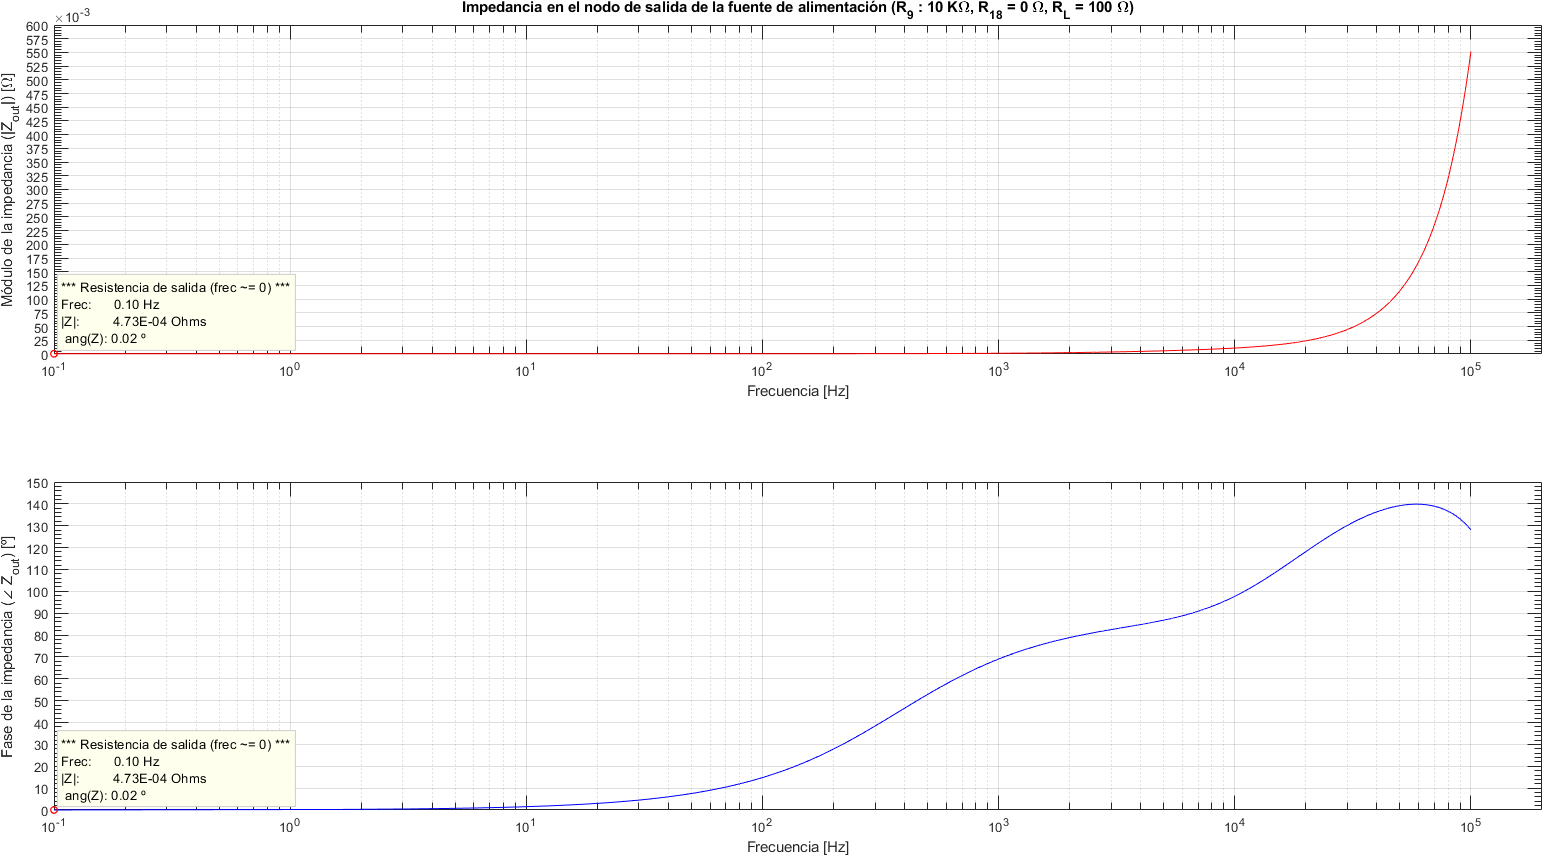
\includegraphics[width=1.2 \textwidth, angle=90]{./img/preguntas/p13.png}
\caption{\label{fig:fig_p13_output_impedance}\footnotesize{Impedancia de salida, $Z_{o}$, en función de la frecuencia, con esta variando entre $0.1 \si[per-mode=symbol]{\hertz}$ y $100 \si[per-mode=symbol]{\kilo\hertz}$.}}
\end{center}
\end{figure}



\clearpage


\subsection{Punto 14}

\textbf{Enunciado}: \textsl{Hallar por simulación la impedancia de la malla de salida en función de la frecuencia para frecuencias desde $0,1 \si[per-mode=symbol]{\hertz}$ hasta $100 \si[per-mode=symbol]{\kilo\hertz}$ y con  $R_{L} = 0 \si[per-mode=symbol]{\ohm}$. Considerar  $R_{18} = 0 \si[per-mode=symbol]{\ohm}$.}


\vspace{1.5cm}


En la figura~\figref{fig:fig_p14_output_impedance} se muestra el gráfico de la impedancia en el nodo de salida en modo de regulación de corriente, el gráfico se obtuvo simulando en \textbf{SPICE} con la salida cortocircuitada a través de una fuente de tensión de señal, $V_{p}$, realizando un barrido en alterna de $0.1 \si[per-mode=symbol]{\hertz}$ a $100 \si[per-mode=symbol]{\kilo\hertz}$, con el comando \textbf{SPICE} \textit{.ac}, y luego obteniendo el cociente $\frac{V_{p}}{I\left({V_{p}}\right)}$, el resultado se exportó y se graficó en \textbf{MATLAB}, en escala semilogarítmica, su módulo y su fase, se destacó el resultado a bajas frecuencias que representa la resistencia de salida a frecuencia bajas/medias. El bajo valor obtenido para esta resistencia ($958 \si[per-mode=symbol]{\ohm}$) implica que no se trata de una buena fuente de corriente, que en el caso ideal tiene resistencia de salida $\infty$, esto se debe a la menor ganancia de lazo en modo regulación de corriente respecto al modo regulación tensión. Otra cosa que se puede observar es que al aumentar la frecuencia la impedancia disminuye, al caer la ganancia de lazo, y se torna capacitiva.




\vfill

\clearpage

\begin{figure}[H] %htb
\begin{center}
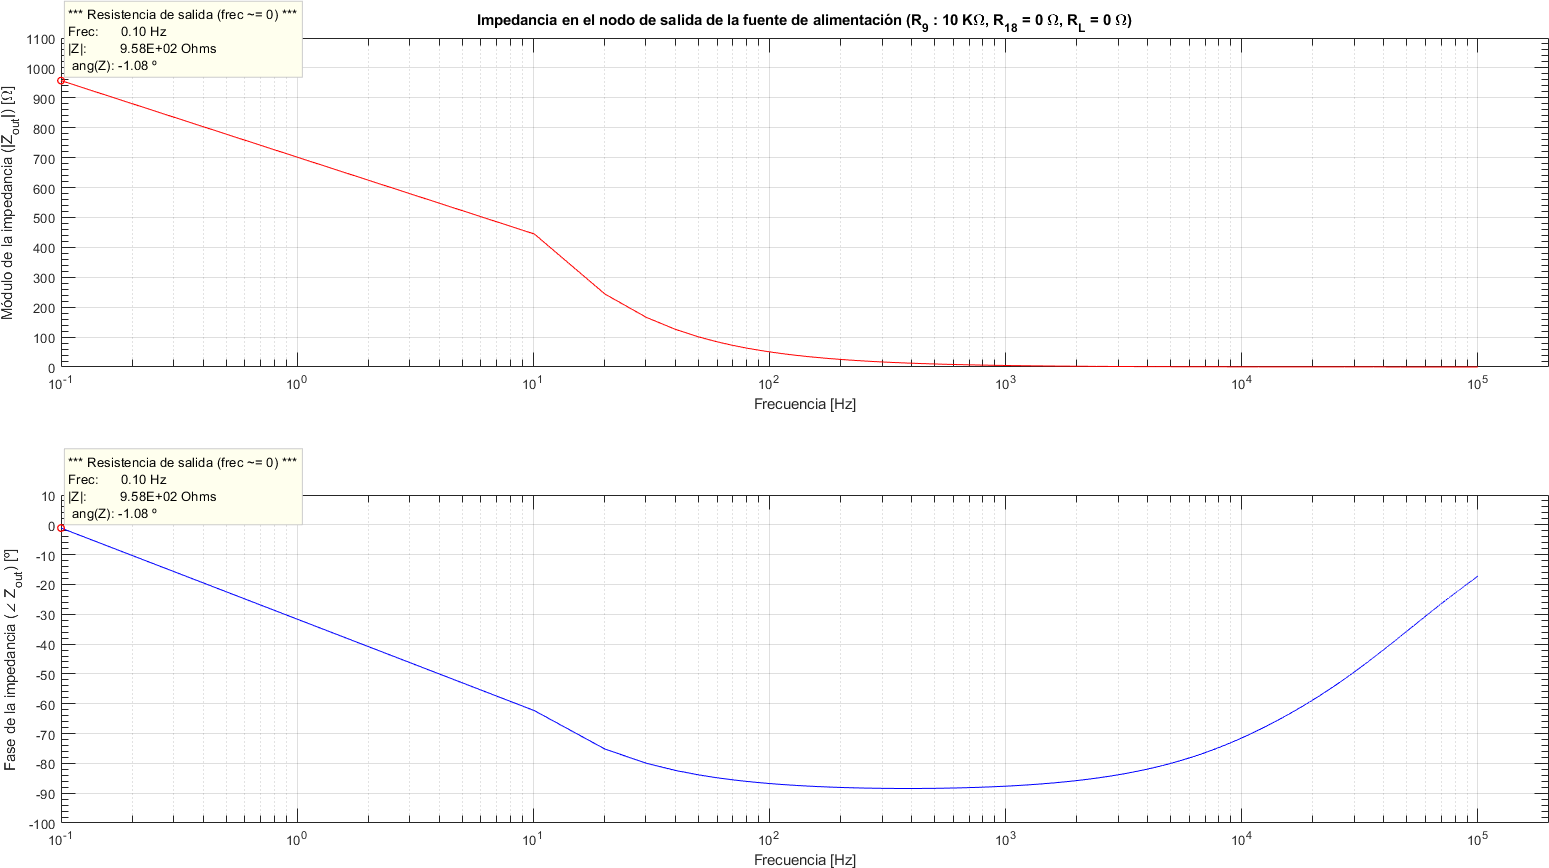
\includegraphics[width=1.2 \textwidth, angle=90]{./img/preguntas/p14.png}
\caption{\label{fig:fig_p14_output_impedance}\footnotesize{Impedancia de salida, $Z_{o}$, en función de la frecuencia, con esta variando entre $0.1 \si[per-mode=symbol]{\hertz}$ y $100 \si[per-mode=symbol]{\kilo\hertz}$.}}
\end{center}
\end{figure}



\clearpage


\subsection{Punto 15}

\textbf{Enunciado}: \textsl{Hallar por simulación la tensión del nodo de salida en función de la corriente de salida para  $R_{L}$ variando entre  $100 \si[per-mode=symbol]{\ohm}$ y $0 \si[per-mode=symbol]{\ohm}$. Considerar $R_{9} = 10 \si[per-mode=symbol]{\kilo\ohm}$ y $R_{18} = 0 \si[per-mode=symbol]{\ohm}$.}


\vspace{1.5cm}


En la figura~\figref{fig:fig_p15_voltage_vs_current} se muestra la variación de la tensión de salida en función de la corriente de salida, se distinguen claramente y están marcadas, las regiones de regulación de tensión (la tensión nominal esperada es de $2 \si[per-mode=symbol]{\volt}$) y corriente (la corriente esperada es de $2 \si[per-mode=symbol]{\ampere}$).




\vfill

\clearpage

\begin{figure}[H] %htb
\begin{center}
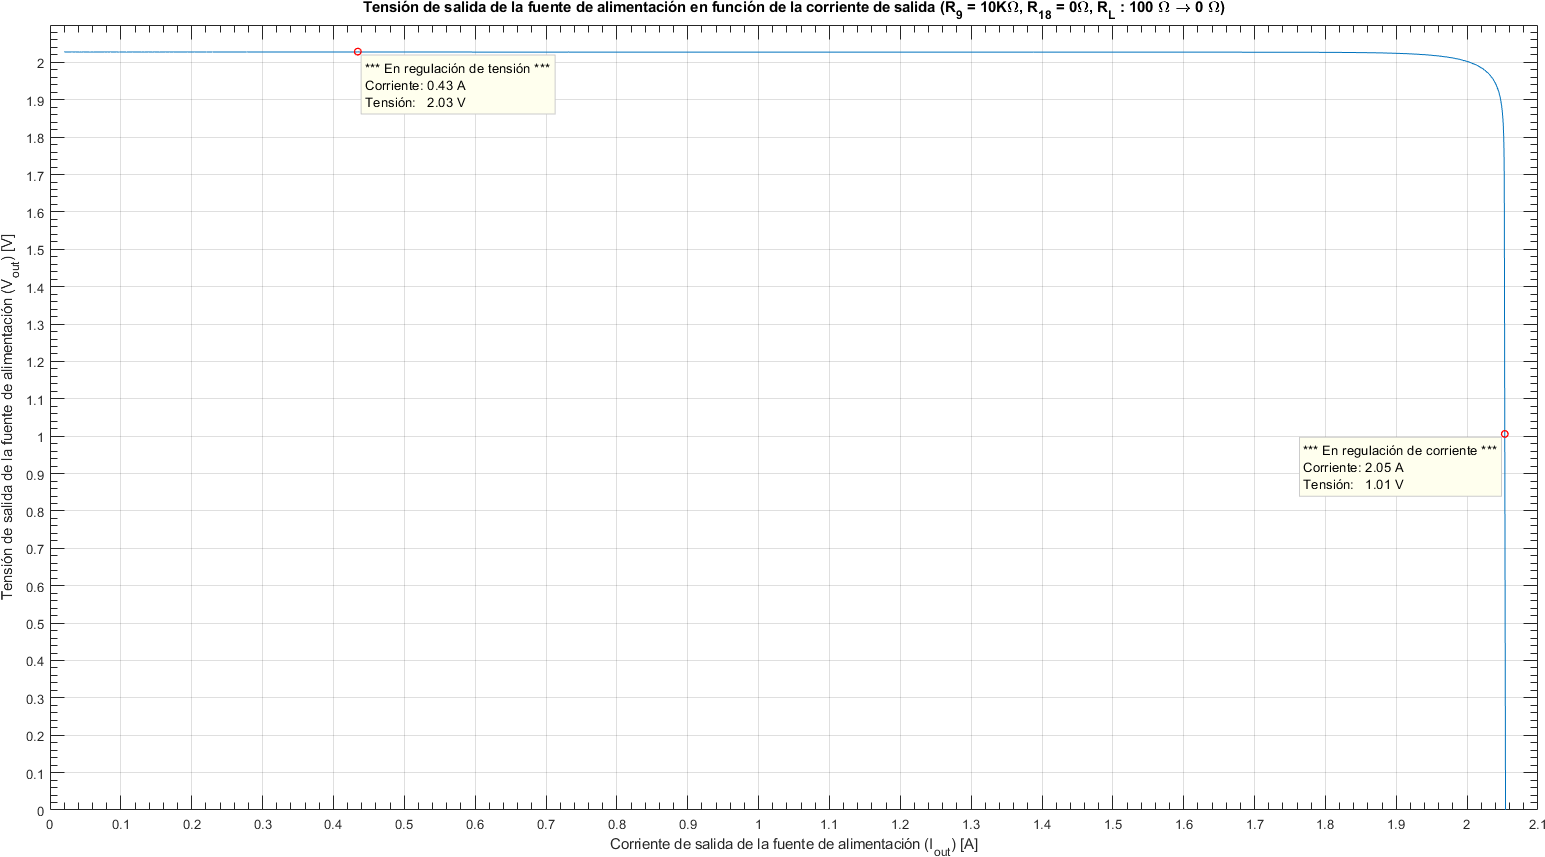
\includegraphics[width=1.2 \textwidth, angle=90]{./img/preguntas/p15.png}
\caption{\label{fig:fig_p15_voltage_vs_current}\footnotesize{Tensión de salida en función de la corriente de salida para $R_{L}$ variando entre $100 \si[per-mode=symbol]{\ohm} y 0 \si[per-mode=symbol]{\ohm}$.}}
\end{center}
\end{figure}



\clearpage



\subsection{Punto 16}

\textbf{Enunciado}: \textsl{Hallar por simulación la variación de la tensión de salida en función del tiempo para un salto abrupto de la corriente de salida desde aproximadamente $0 \si[per-mode=symbol]{\ampere}$ hasta $ 1 \si[per-mode=symbol]{\ampere}$ y posteriormente un salto abrupto de la corriente de salida desde aproximadamente $ 1A$ hasta $0 A$. Considerar $R_{9} = 10 \si[per-mode=symbol]{\kilo\ohm}$ y $R_{18} = 0 \si[per-mode=symbol]{\ohm}$.}


\vspace{1.5cm}


Para lograr la conmutación de la carga se utilizó el circuito mostrado en la figura~\figref{fig:fig_p16_rl_switch}, donde se puede ver el modelo de una llave controlada por tensión con resistencia de $0 \si[per-mode=symbol]{\ohm}$ en estado cerrado y resistencia tendiendo a infinito (valor muy grande) para el estado abierto. El switch es controlado por una onda cuadrada, de tal manera de lograr una carga de $0 \si[per-mode=symbol]{\ampere}$ al comienzo de la simulación, de $1 \si[per-mode=symbol]{\ampere}$ ($R_{L} = 2 \si[per-mode=symbol]{\ohm}$) a los $20 \si[per-mode=symbol]{\milli\second}$, y luego nuevamente $0 \si[per-mode=symbol]{\ampere}$ a los $50 \si[per-mode=symbol]{\milli\second}$. La simulación realizada es del tipo transitorio (\textbf{SPICE} \textit{.tran}), la salida de la misma se muestra resaltando el momento de las transiciones en la figura~\figref{fig:fig_p16_output_in_load_jump}. En la figura~\figref{fig:fig_p16_output_variation_in_load_jump} se destaca la diferencia en la tensión de salida en carga respecto a en vacío, esta diferencia permite estimar la resistencia de salida de la fuente de alimentación, el valor obtenido es:\\


\begin{equation}
R_{o} = \frac{\Delta V}{\Delta I} = \frac{\num{3.67E-4} \si[per-mode=symbol]{\volt}}{1.0137 \si[per-mode=symbol]{\ampere}} = 642 \si[per-mode=symbol]{\micro\ohm}
\end{equation}

\begin{figure}[H] %htb
\begin{center}
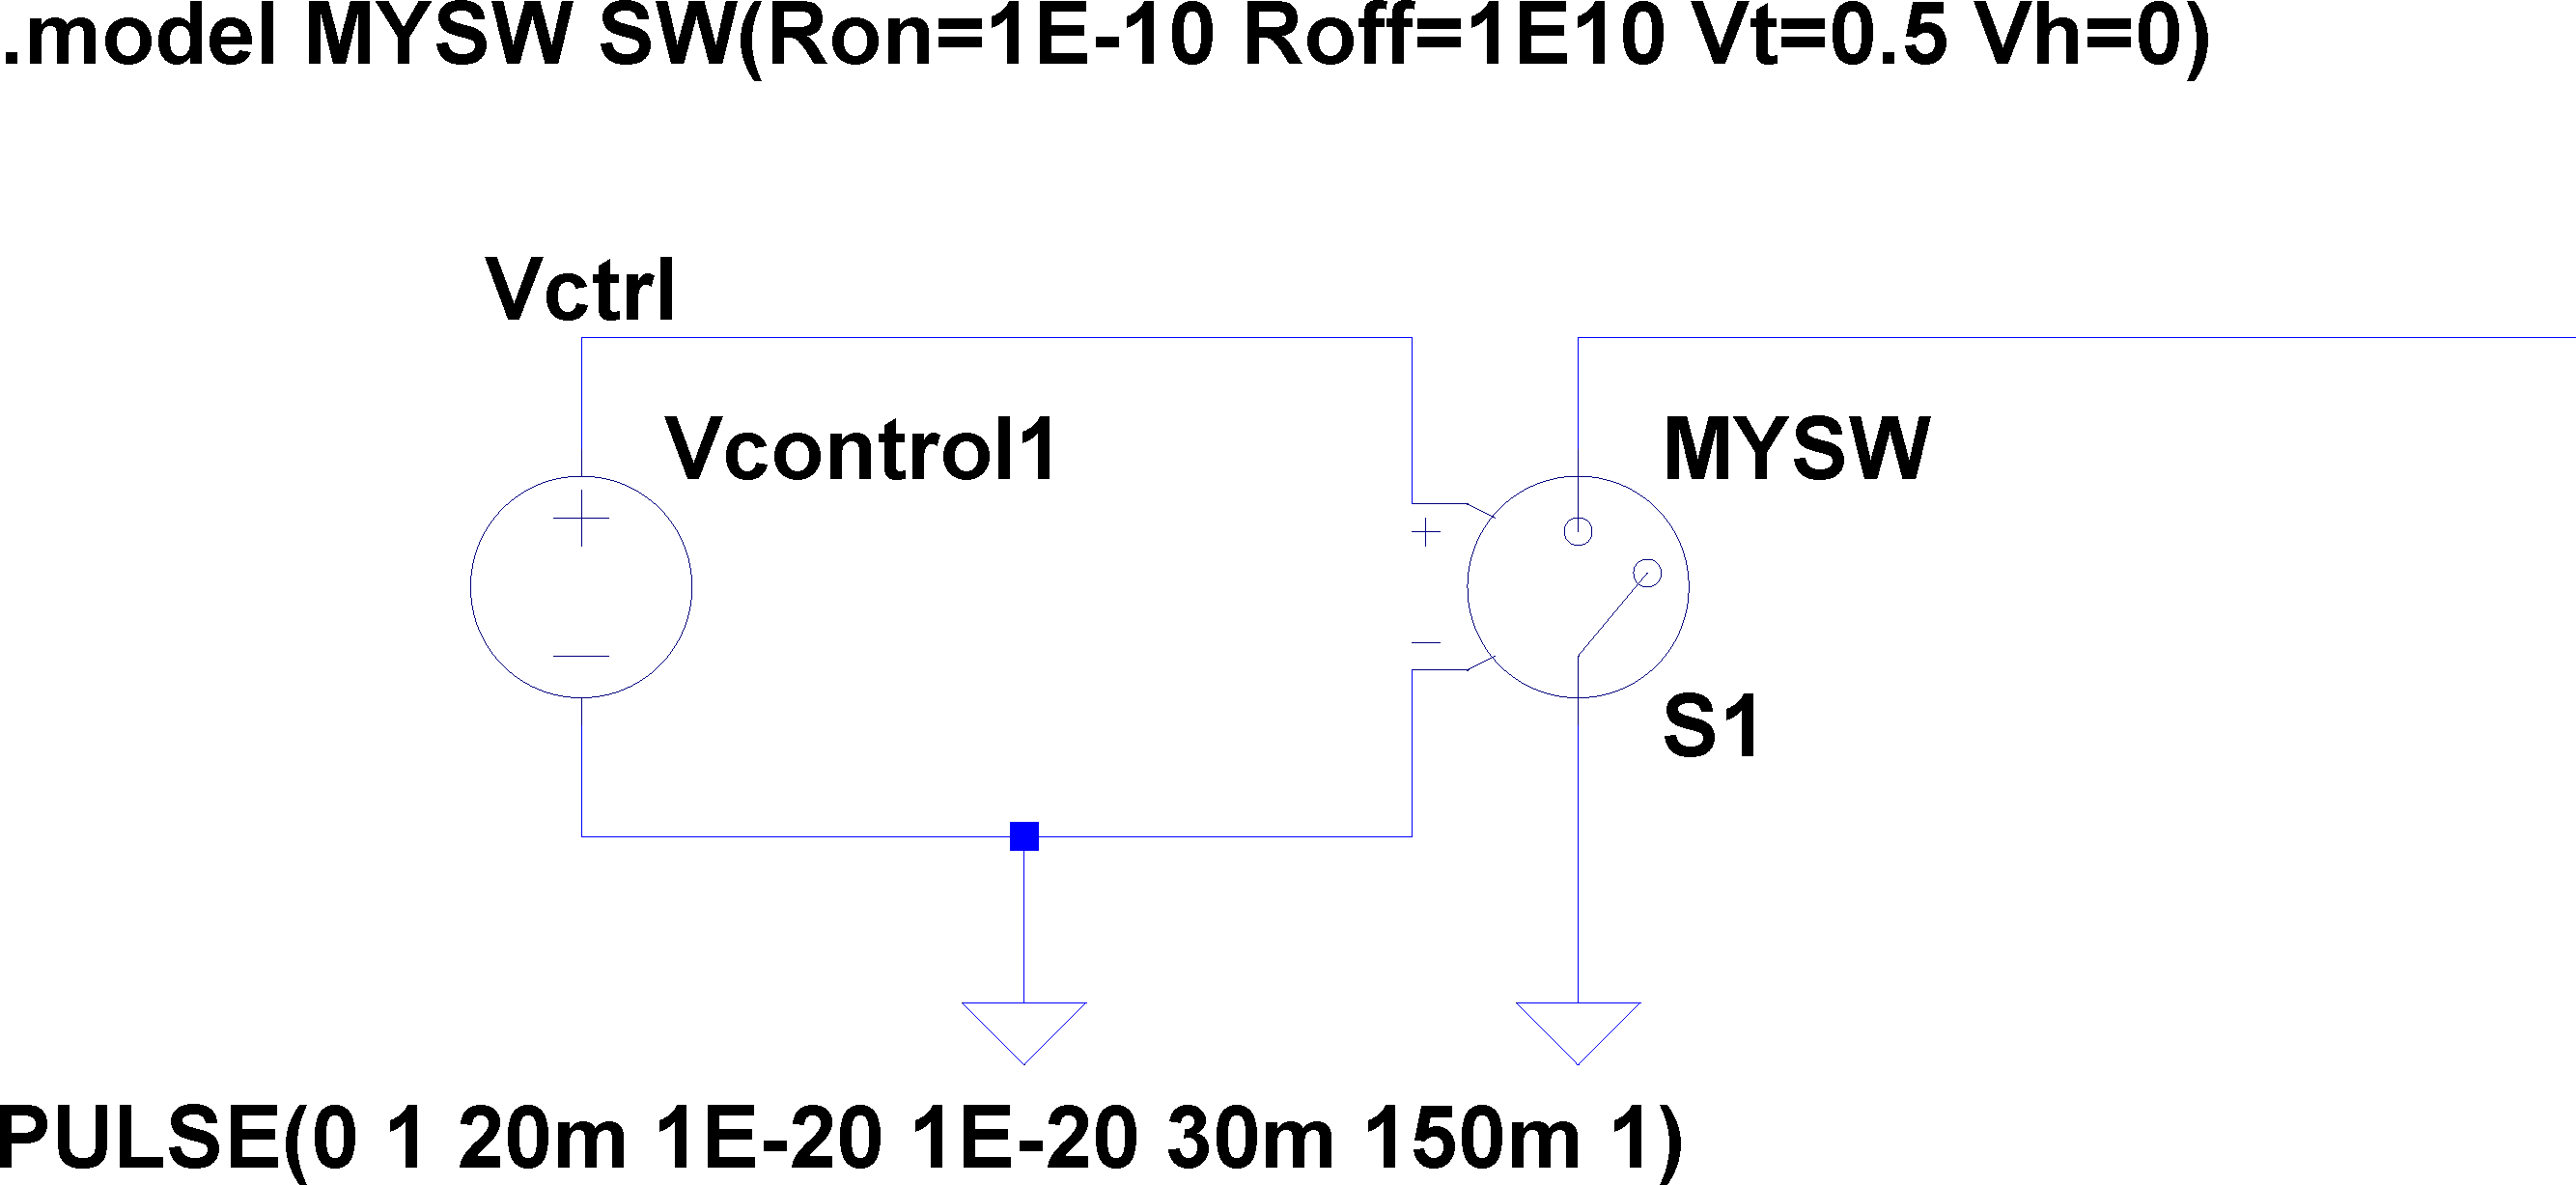
\includegraphics[width=0.9 \textwidth, angle=0]{./img/preguntas/p16a.png}
\caption{\label{fig:fig_p16_rl_switch}\footnotesize{Circuito usado para la conmutación de la carga}}
\end{center}
\end{figure}


\vfill

\clearpage

\begin{figure}[H] %htb
\begin{center}
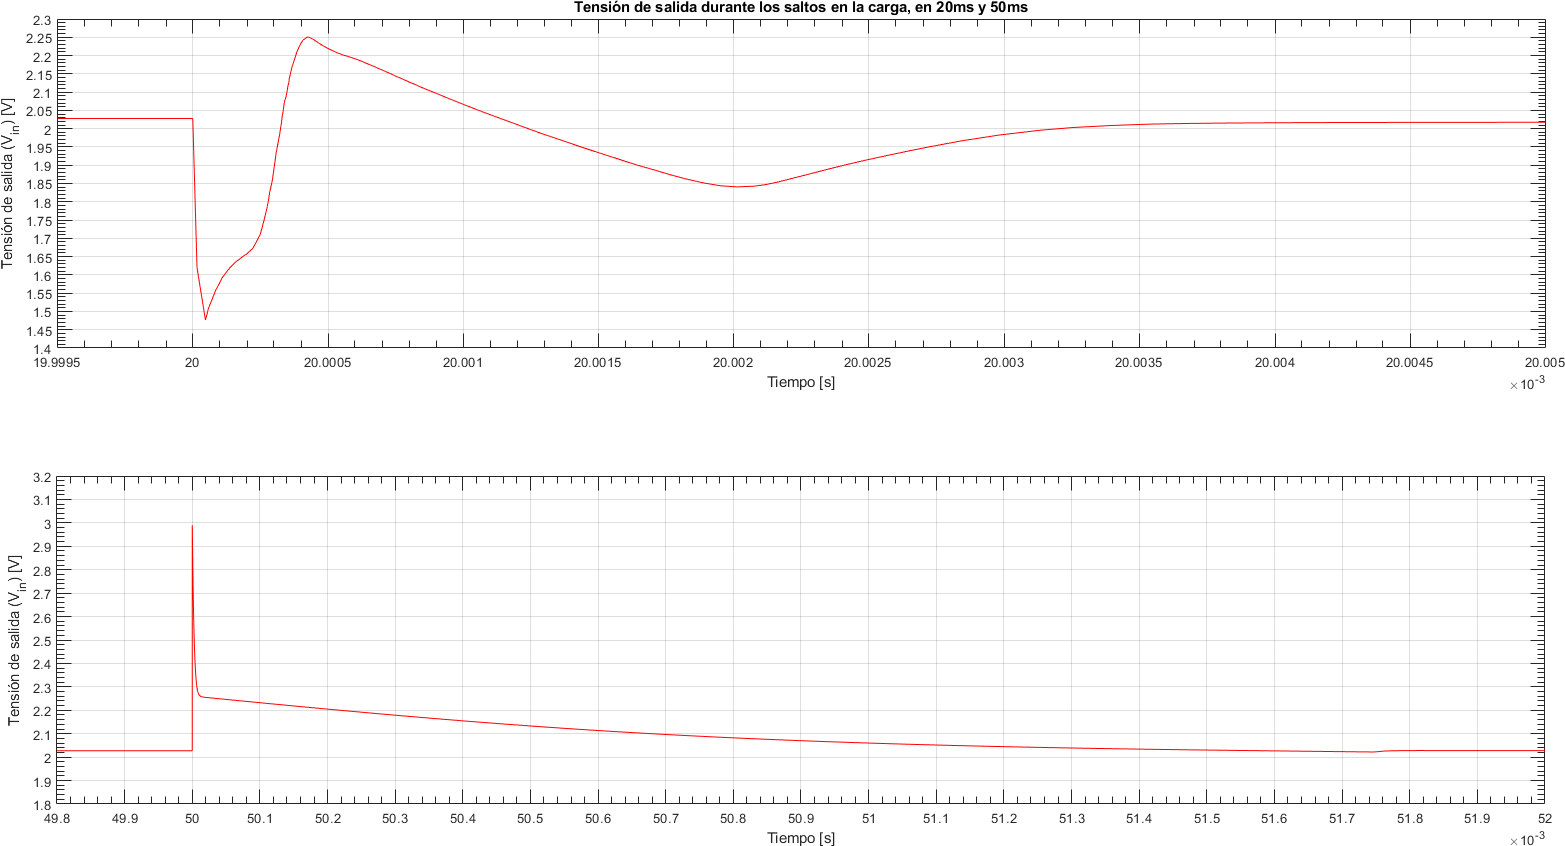
\includegraphics[width=1.2 \textwidth, angle=90]{./img/preguntas/p16b.png}
\caption{\label{fig:fig_p16_output_in_load_jump}\footnotesize{Tensión de salida frente a saltos de carga de $0 \si[per-mode=symbol]{\ampere}$ a $1 \si[per-mode=symbol]{\ampere}$ y de $1 \si[per-mode=symbol]{\ampere}$ a $0 \si[per-mode=symbol]{\ampere}$.}}
\end{center}
\end{figure}


\clearpage

\begin{figure}[H] %htb
\begin{center}
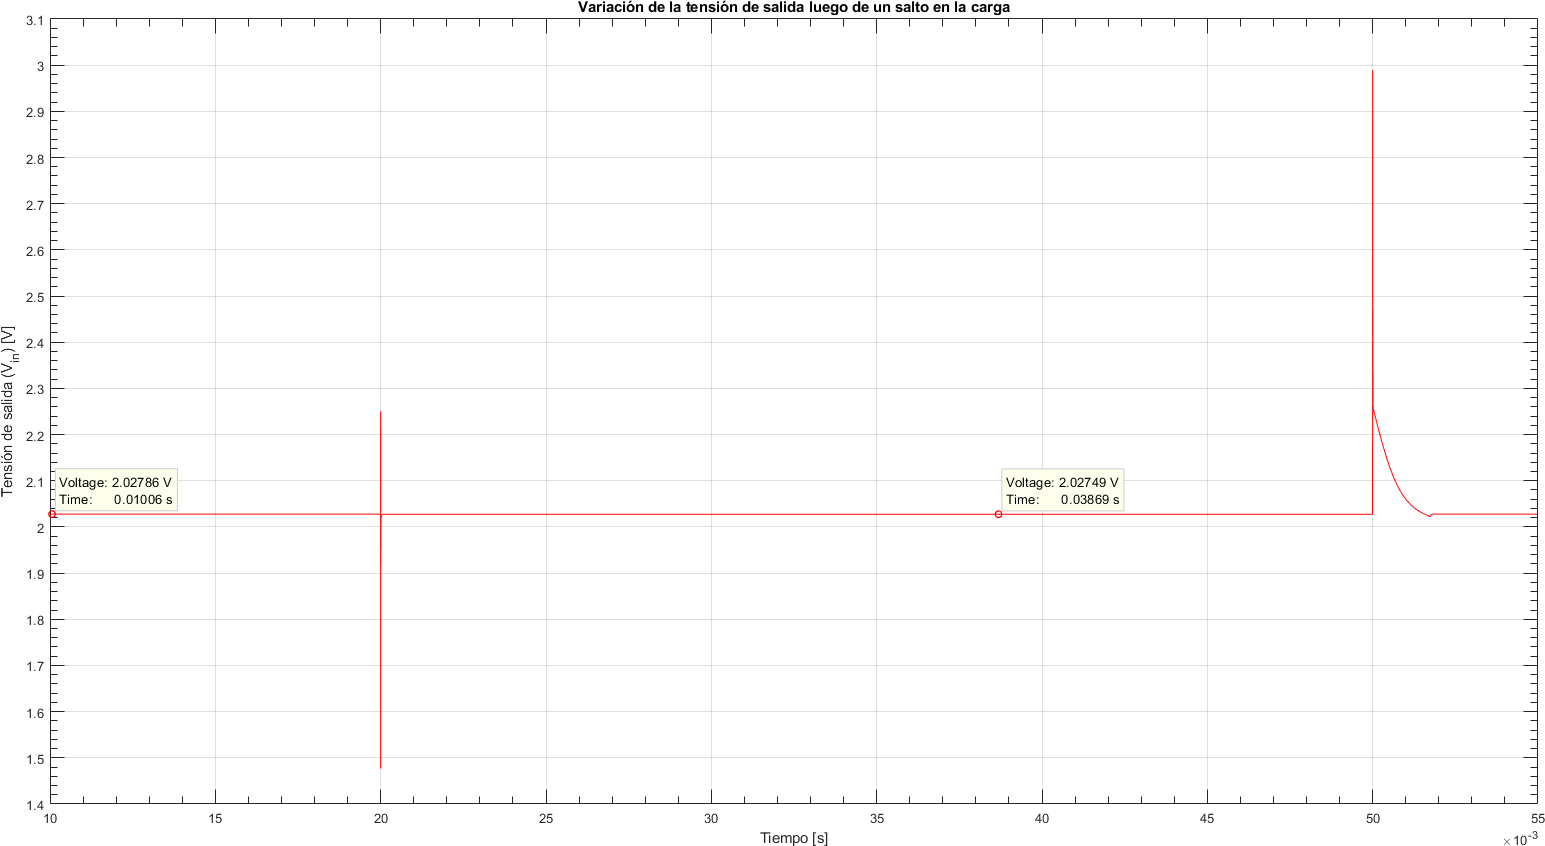
\includegraphics[width=1.2 \textwidth, angle=90]{./img/preguntas/p16c.png}
\caption{\label{fig:fig_p16_output_variation_in_load_jump}\footnotesize{Variación de la tensión de salida en los saltos de carga}}
\end{center}
\end{figure}




\clearpage


\subsection{Punto 17}

\textbf{Enunciado}: \textsl{Calcular la eficiencia para $V_{1}$ igual a $15 \si[per-mode=symbol]{\volt}$, $20 \si[per-mode=symbol]{\volt}$ y $25 \si[per-mode=symbol]{\volt}$.}

\begin{enumerate}
\item[\textsl{a)}] \textsl{con} $R_{L} = 10 \si[per-mode=symbol]{\ohm}$, $R_{9} = 90 \si[per-mode=symbol]{\kilo\ohm}$ y $R_{18} = 0 \si[per-mode=symbol]{\ohm}$.
\item[\textsl{b)}] \textsl{con} $R_{L} = 1 \si[per-mode=symbol]{\ohm}$, $R_{9} = 0 \si[per-mode=symbol]{\ohm}$ y $R_{18} = 0 \si[per-mode=symbol]{\ohm}$.
\end{enumerate}


\vspace{1.5cm}

Para calcular la eficiencia de la fuente de alimentación simplemente se aplicó la definición $\eta = \frac{P_{out}}{P_{in}}$, el cálculo se realizó en estado estacionario, ignorando el consumo durante los transitorios, los cuales de todas formas, a largo plazo, deben ser despreciables. El cálculo se realizó directamente dentro del \textbf{LTSPICE}, utilizando el comando de \textbf{SPICE}, \textit{.measure}, este comando permite realizar cálculos utilizando valores de variables simuladas, y luego operar con estos resultados. Realizando una simulación de \textbf{SPICE} de punto de operación, \textit{.op}, se realizan las siguientes mediciones:

%******************************************************************************************
\lstset{language=,xleftmargin=1em,numbers=none}

\lstset{showspaces=false}
\lstset{showstringspaces=false}
\normalfont
\normalsize
\lstset{backgroundcolor=\color{white},rulecolor=\color{blue}}
\lstset{basicstyle=\ttfamily\color{Deepblue}}

\lstset{keywordstyle=[1]\ttfamily\color{red}\bfseries}
\lstset{keywordstyle=[2]\ttfamily\color{LightSkyBlue}}
\lstset{keywordstyle=[3]\ttfamily\bfseries\color{Plum}}
\lstset{keywordstyle=[4]\ttfamily\bfseries\color{Chocolate}}

\lstset{identifierstyle=\ttfamily\color{black}}
\lstset{commentstyle=\ttfamily\color{blue}\textit}
\lstset{stringstyle=\ttfamily\color{purple}\upshape}
\lstset{tabsize=4}

\lstset{numberstyle=\ttfamily\color{Deeppurple}\upshape}
\lstset{numbersep=5pt}

\lstset{inputencoding=utf8/latin1}



\fontencoding{T1}
\fontseries{m}
\fontsize{10pt}{11pt}
\selectfont
%******************************************************************************************


\begin{lstlisting}
.op

.meas Pin PARAM V(Vin)*(-I(V1))
.meas Pout PARAM V(Vout)*(-I(RL))
.meas Eff PARAM Pout / Pin
\end{lstlisting}



Los resultados obtenidos para la eficiencia para cada uno de los valores de tensión de entrada para la que se realizó la simulación, se resumen en la tabla~\tableref{table:table_efficiency}. Se puede ver claramente como la eficiencia disminuye al aumentar la diferencia entre la tensión de entrada y la tensión de salida, cosa totalmente esperable, ya que, a tensión de salida constante, la tensión en el elemento de paso es cada vez mayor, a la misma corriente de carga, se tiene mayor potencia disipada en el mismo.\\
También la eficiencia empeora con el aumento de la carga, ya que al pasar la corriente de carga por el elemento de paso. se disipará también mas potencia en este.\\

%% \noindent
%% \begin{center}
 
%%\begin{spacing}{1}  
\bgroup
\begin{table}[H]  %%\centering
    
    \setlength\arrayrulewidth{1.5pt}
    \arrayrulecolor{white}
    \def\clinecolor{\hhline{|>{\arrayrulecolor{white}}-%
    >{\arrayrulecolor{white}}|-|-|-|-|}}
\resizebox{0.9 \textwidth}{!}{% 
       
\def\arraystretch{2.5}
\begin{tabularx}{1 \textwidth}%
    {|
    >{\columncolor{white} \centering\arraybackslash}m{0.25\linewidth}
     |
    >{\columncolor{white} \centering\arraybackslash}m{0.25\linewidth}
     |
    >{\columncolor{white} \centering\arraybackslash}m{0.25\linewidth}
     |
    >{\columncolor{white} \centering\arraybackslash}m{0.25\linewidth}
     |
    }
    \rowcolor{HeadersColor} \cellcolor{white} \thead{}  & \thead{$V_{i} = 15 \si[per-mode=symbol]{\volt}$} & \thead{$V_{i} = 20 \si[per-mode=symbol]{\volt}$} & \thead{$V_{i} = 25 \si[per-mode=symbol]{\volt}$} \\
    
    \hhline{|-|-|-|-|}
    \rowcolor{gray!20} \cellcolor{gray!60} \thead{ \cellcolor{gray!60} $\eta = \frac{P_{out}}{P_{in}} \cdot 100 \%$ \\ \cellcolor{gray!60} \\ \cellcolor{gray!60} $R_{L} = 10 \si[per-mode=symbol]{\ohm}$, $R_{9} = 90 \si[per-mode=symbol]{\kilo\ohm}$ \\ \cellcolor{gray!60} $R_{18} = 0 \si[per-mode=symbol]{\ohm}$ } & 63.93 \% & 48.04 \% & 38.50 \%  \\
    \hhline{|-|-|-|-|}
    \rowcolor{gray!20} \cellcolor{gray!60}  \thead{ \cellcolor{gray!60} $\eta = \frac{P_{out}}{P_{in}} \cdot 100 \%$ \\ \cellcolor{gray!60} \\ \cellcolor{gray!60} $R_{L} = 1 \si[per-mode=symbol]{\ohm}$, $R_{9} = 0 \si[per-mode=symbol]{\ohm}$ \\ \cellcolor{gray!60} $R_{18} = 0 \si[per-mode=symbol]{\ohm}$ } & 6.58 \% & 4.95 \% & 3.96 \%  \\
    \hhline{|-|-|-|-|}        
    \end{tabularx}}
	\caption{\footnotesize{Eficiencia en función de la tensión de entrada.}}
	\label{table:table_efficiency}
\end{table}
\egroup
%%\end{spacing}

%% \end{center}



\clearpage

\subsection{Punto 18}

\textbf{Enunciado}: \textsl{¿Cómo influye en la tensión de salida la variación de la fuente de entrada $V_{1}$ (variando de $1 \si[per-mode=symbol]{\volt}$ a $30 \si[per-mode=symbol]{\volt}$ y con $R_{L} = 10 \si[per-mode=symbol]{\ohm}$, $R_{9} = 90 \si[per-mode=symbol]{\kilo\ohm}$ y $R_{18} = 0 \si[per-mode=symbol]{\ohm}$)?. Simular para graficar la tensión de salida en función de $V_{1}$.}\\


\vspace{1.5cm}

Es de esperarse que la fuente tenga un valor mínimo de tensión de entrada, a partir del cual empieza a regular la salida, para valores menores de tensión que este valor mínimo, la salida será menor a la esperada, en principio, el regulador paralelo para regular a $10 \si[per-mode=symbol]{\volt}$, necesita una tensión de entrada mayor, pero también se deben polarizar correctamente los transistores, y como puede verse en la figura~\figref{fig:fig_p18_vo_vs_vi}, el crecimiento de la salida es prácticamente lineal, manteniendo una diferencia de aproximadamente $2.2 \si[per-mode=symbol]{\volt}$ a la salida con respecto a la entrada, este valor sería el \quotemarks{drop-out} de esta fuente de alimentación. Tomando que la salida está regulando al 
llegar a aproximadamente al $1 \%$ de la tensión regulada esperada a la salida, $10 \si[per-mode=symbol]{\volt}$, el valor de tensión de entrada mínimo para salida regulada es de $12.38 \si[per-mode=symbol]{\volt}$. También puede observarse que para tensiones muy pequeñas a la entrada, hasta aproximadamente $1.8 \si[per-mode=symbol]{\volt}$, la tensión a la salida es prácticamente $0 \si[per-mode=symbol]{\volt}$, esto se explica por estar cortado el elemento de paso de la fuente de alimentación, el par compuesto.

\vfill

\clearpage

\begin{figure}[H] %htb
\begin{center}
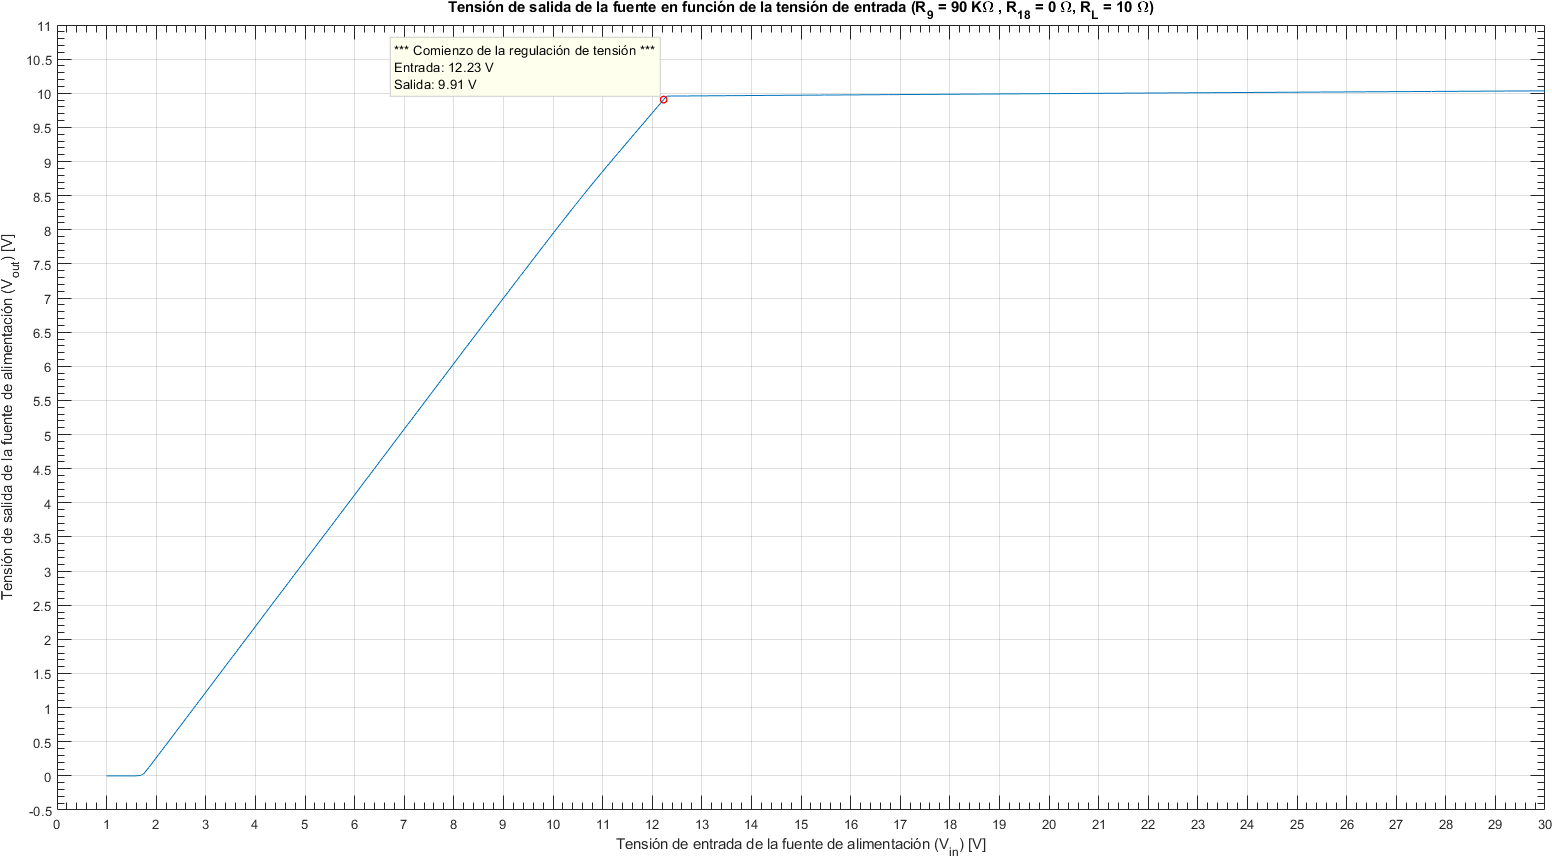
\includegraphics[width=1.2 \textwidth, angle=90]{./img/preguntas/p18.png}
\caption{\label{fig:fig_p18_vo_vs_vi}\footnotesize{Tensión de salida vs tensión de entrada.}}
\end{center}
\end{figure}

\clearpage


\subsection{Punto 19}

\textbf{Enunciado}: \textsl{¿Cómo influye en la corriente de salida la variación de la fuente de entrada $V_{1}$ (variando de $1 \si[per-mode=symbol]{\volt}$ a $30 \si[per-mode=symbol]{\volt}$ y con $R_{L} = 0 \si[per-mode=symbol]{\ohm}$, $R_{9} = 90 \si[per-mode=symbol]{\kilo\ohm}$ y $R_{18} = 0 \si[per-mode=symbol]{\ohm}$?. Simular para graficar la corriente de salida en función de $V_{1}$.}\\

\vspace{1.5cm}

De la misma forma que el punto anterior, es de esperarse que la fuente tenga un valor mínimo de tensión de entrada, a partir del cual empieza a regular la salida, para valores menores de tensión que este valor mínimo, la corriente de salida será solo limitada a algún valor menor al esperado, y como puede verse en la figura~\figref{fig:fig_p19_io_vs_vi}, el crecimiento de la salida es prácticamente lineal, salvo que se produce un pico de corriente alrededor de los $3 \si[per-mode=symbol]{\volt}$ de entrada, que es limitado por la acción de $Q_{15}$, a ese valor de tensión de entrada el lazo de corriente seguramente no actúa de ninguna forma para limitar la corriente de salida. Tomando que la salida está regulando al llegar a aproximadamente al $1 \%$ de la corriente regulada esperada a la salida, $2.05 \si[per-mode=symbol]{\ampere}$, el valor de tensión de entrada mínimo para salida regulada es de $12.19 \si[per-mode=symbol]{\volt}$, valor muy cercano al del punto anterior. También puede observarse que para tensiones muy pequeñas a la entrada, aproximadamente $1.8 \si[per-mode=symbol]{\volt}$, la corriente a la salida es prácticamente $0 A$, esto se explica por la misma razón que en el punto anterior.

\vfill

\clearpage

\begin{figure}[H] %htb
\begin{center}
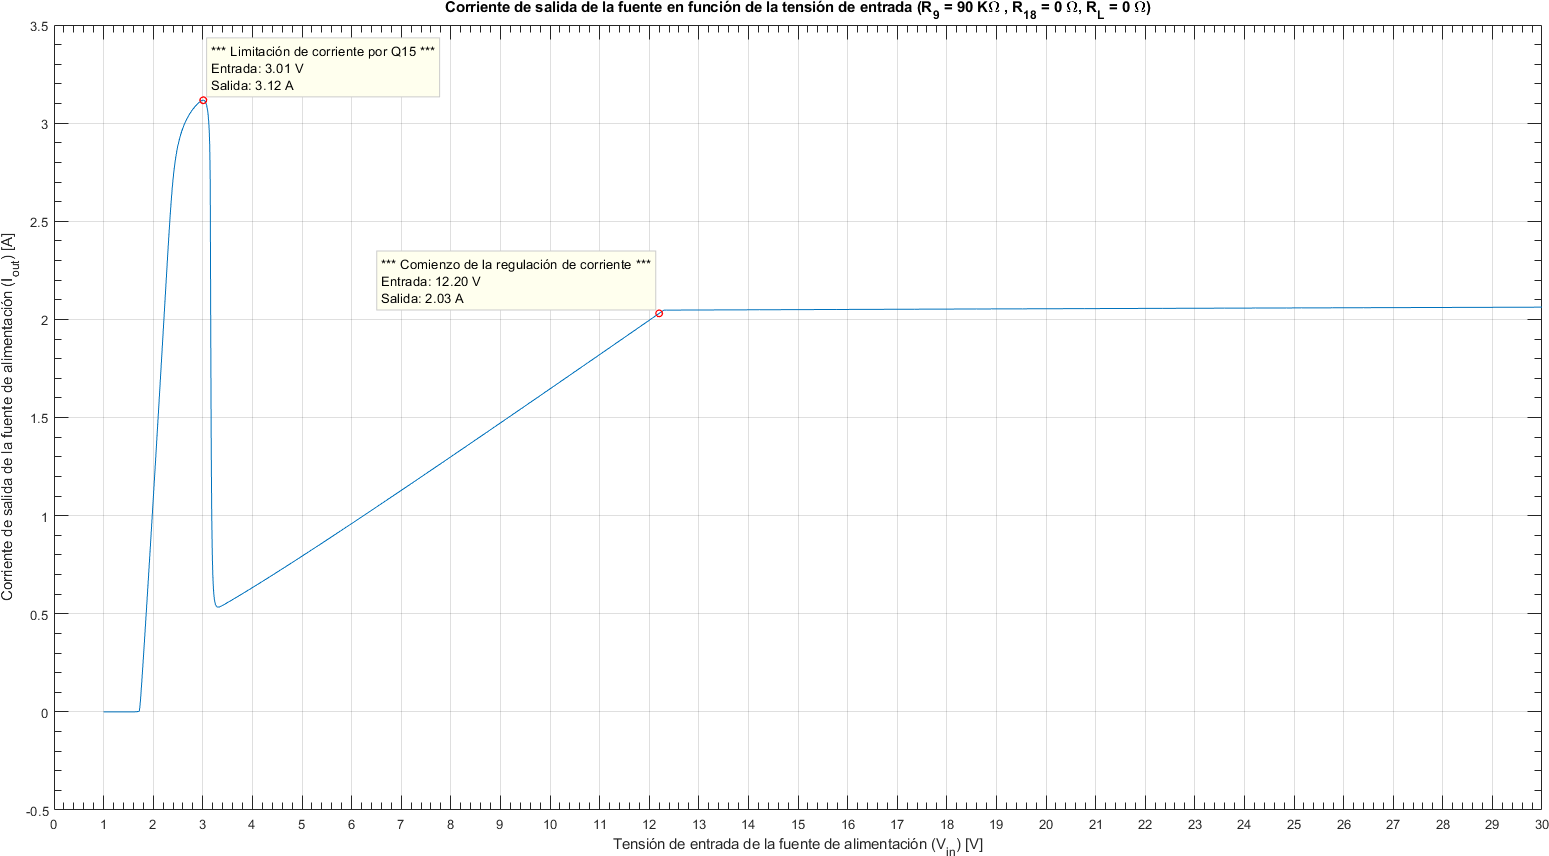
\includegraphics[width=1.2 \textwidth, angle=90]{./img/preguntas/p19.png}
\caption{\label{fig:fig_p19_io_vs_vi}\footnotesize{Tensión de salida vs tensión de entrada.}}
\end{center}
\end{figure}

\clearpage


\subsection{Punto 20}

\textbf{Enunciado}: \textsl{Determinar el rechazo de ruido, o sea, ¿Cuántos decibles de diferencia se miden comparando un ruido presente en la tensión de entrada $V_{1}$ respecto del residuo de ese ruido en la tensión de salida. Debe intentarse no considerar el ruido propio de la fuente. \textbf{NOTA}: el ruido podría ser por ejemplo el rizado resultante de una rectificación y filtrado.}\\



Para ver el rechazo de ruido que presenta la fuente de alimentación, sumamos a la tensión de entrada una señal en forma de diente de sierra descendente de $100 Hz$, ya que la sugerencia era que el ruido podría provenir del rizado resultante de una rectificación y filtrado. Se utilizó una señal de $2 V$ de amplitud para poder apreciar bien la amplitud de la señal en la salida. Se graficó la entrada y la salida restándole la tensión continua de base, $20 V$ a la entrada y el valor mínimo a la salida, alrededor de $2 V$, se utilizó un script de \textbf{MATLAB} para restar los valores adecuados, hacer los cálculos y producir los gráficos a partir de los datos exportados del \textbf{LTSPICE}. En la figura~\figref{fig:fig_p20_ripple}, se muestra lo obtenido, mostrando simultáneamente 2 ciclos del rizado de entrada y salida.
Como se observa en la figura, la salida presenta un cierto tiempo de crecimiento debido al ancho de banda limitado del amplificador de la fuente, y presenta además un pequeño pico en la discontinuidad, el mismo se debe al tipo de compensación del circuito, tema que veremos en la siguiente parte del trabajo práctico. Si se mide el rechazo de ruido simplemente como el cociente de valor RMS de la señal de salida respecto de la entrada obtenemos:


\begin{equation}
    R_{nr}= 59.49 dB
\end{equation}

Sin embargo se pedía intentar no considerar el ruido propio de la fuente, entonces lo que se hizo fue, extrapolar la amplitud máxima de la señal de rizado a la salida, ignorando el sobre-pico y el tiempo de crecimiento, midiendo su amplitud cerca de la mitad de la amplitud máxima de la señal de entrada, calculado así, obtuvimos:


\begin{equation}
    R_{nr}= 61.41 dB
\end{equation}

\vfill

\clearpage

\begin{figure}[H] %htb
\begin{center}
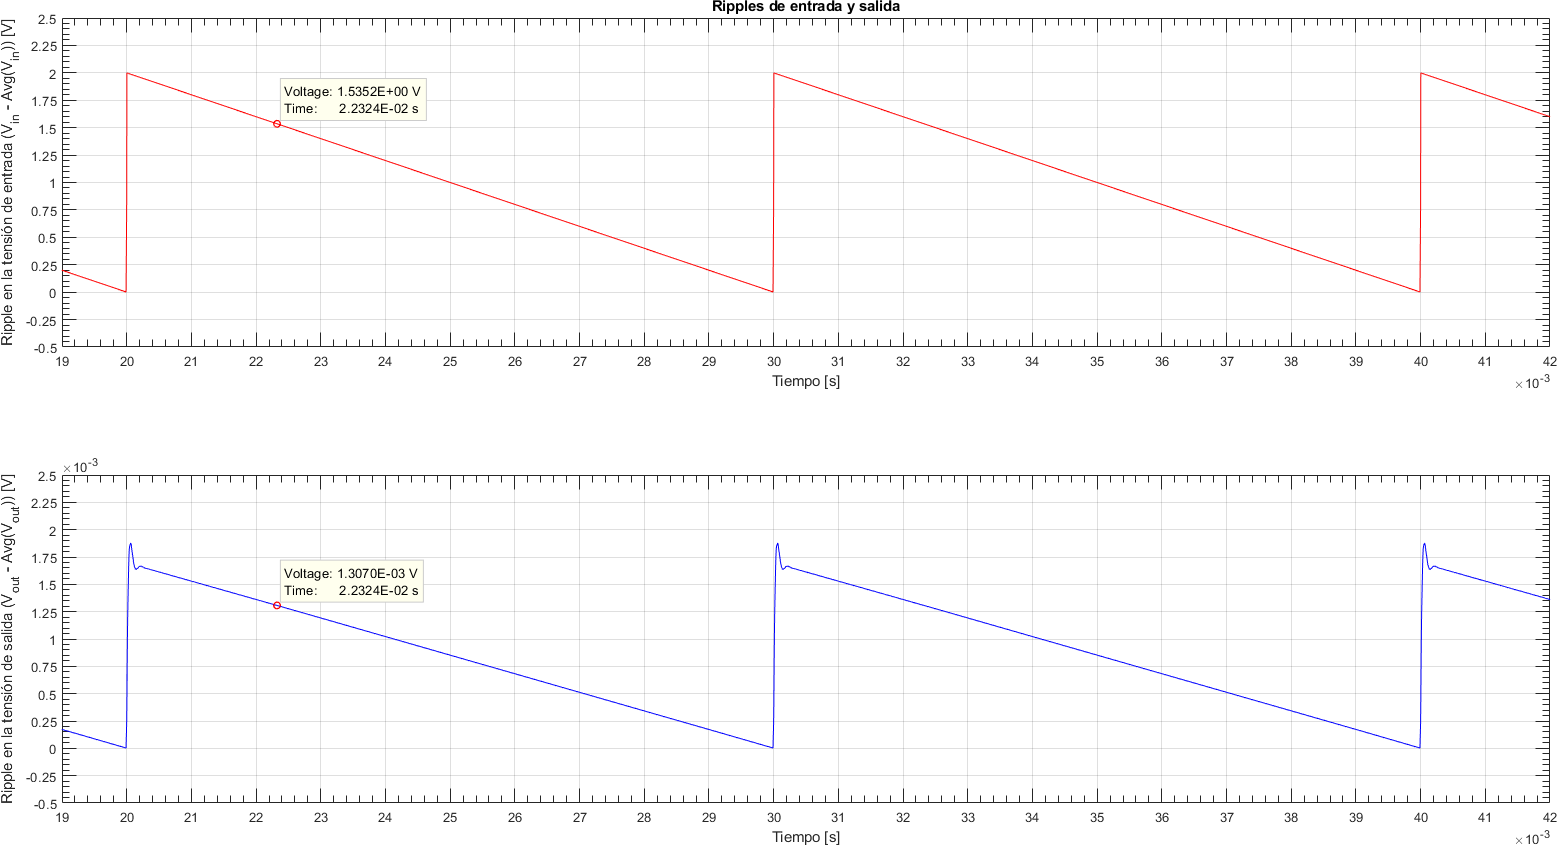
\includegraphics[width=1.2 \textwidth, angle=90]{./img/preguntas/p20.png}
\caption{\label{fig:fig_p20_ripple}\footnotesize{Rizado de entrada y salida.}}
\end{center}
\end{figure}

\clearpage


\clearpage

\subsection{Punto 21}

Modificar el circuito de la fuente reemplazando en parte o totalmente el amplificador por el regulador integrado $LM723$ y evaluar el comportamiento del nuevo diseño comparándolo con el original.

\clearpage


